% Scientific supplement. Regenerate the literature note with revision/build_references.py.
\documentclass[10pt,letterpaper]{article}
\usepackage[margin=0.80in]{geometry}
\usepackage{amsmath,amssymb,amsthm,graphicx,booktabs,longtable,array}
\usepackage{placeins}
\usepackage[font=small,labelfont=bf,labelsep=period]{caption}
\usepackage[hidelinks]{hyperref}
\urlstyle{same}
\setlength{\emergencystretch}{2em}
\setlength{\parindent}{1em}
\setlength{\LTpre}{0.5em}
\setlength{\LTpost}{0.5em}
\renewcommand{\theequation}{\arabic{equation}}
\renewcommand{\thefigure}{\arabic{figure}}
\renewcommand{\thetable}{\arabic{table}}
\renewcommand{\figurename}{Supplementary Figure}
\renewcommand{\tablename}{Supplementary Table}
\makeatletter
\def\input@path{{supplementary/}}
\def\section@cntformat{Supplementary Note\ \thesection.\quad}
\renewcommand{\@seccntformat}[1]{\@ifundefined{#1@cntformat}{\csname the#1\endcsname\quad}{\csname #1@cntformat\endcsname}}
\makeatother
\raggedbottom
\hypersetup{pdftitle={Supplementary Information for Bounding the rate loss of individual paired wireless uplink schedules},pdfauthor={Pooya Hejazi and Masoud Sabaei}}
\begin{document}
\begin{center}
{\Large\bfseries Supplementary Information\par}
\medskip
{\large Bounding the rate loss of individual paired wireless uplink schedules\par}
\medskip
Pooya Hejazi and Masoud Sabaei
\end{center}
\noindent The seven notes give the mathematical derivations, numerical enclosures, solver specification, extended simulations and measurement processing underlying the Article. Rates are normalized per occupied tone in bit/s/Hz unless stated as aggregate nats. Supplementary Tables 1--16 and Supplementary Figures 1--8 retain the observation units and computational scope of their source experiments.
\section{Comparison with closely related work}
\label{suppnote:literature}
The comparison identifies the model and guarantee supplied by each approach. Matching, continuous enclosures and conformal ranks are established ingredients; their roles in the present action-specific interval are distinguished below.
\begin{table}[htbp]\centering\small
\setlength{\tabcolsep}{3pt}
\caption{Ten closely related studies and their relation to the paired scheduling interval.}\label{supp:comparison}
\begin{tabular}{@{}>{\raggedright\arraybackslash}p{.14\linewidth}>{\raggedright\arraybackslash}p{.20\linewidth}>{\raggedright\arraybackslash}p{.21\linewidth}>{\raggedright\arraybackslash}p{.19\linewidth}>{\raggedright\arraybackslash}p{.20\linewidth}@{}}\toprule
Study & System and receiver & Optimization / learning & Guarantee & Relation to this work\\\midrule
Viterbo and Hottinen~\cite{viterbo} & Equal-energy paired uplink; MMSE/ML detection & Optimal pairing & Optimum in its pairing model & Tone-dependent conflicts and continuous powers\\\addlinespace[3pt]
Fan et al.~\cite{fan} & LTE uplink; linear MMSE & Pairing and contiguous allocation & Discrete search with prescribed powers & Full power-domain ceiling for a delivered action\\\addlinespace[3pt]
Ruder et al. (2013)~\cite{ruder2013} & SC-FDMA; receiver-specific metrics & Blossom pairing and joint grouping & Small full-enumeration benchmark & Scalable checked relaxation across labelled tones\\\addlinespace[3pt]
Ruder et al. (2014)~\cite{ruder2014} & SC-FDMA; imperfect scheduling CSI & MMSE prediction and grouping & Small perfect-CSI search benchmark & Calibrated errors along stored receive directions\\\addlinespace[3pt]
Prasad et al.~\cite{prasad} & LTE-A; matroid/knapsack constraints & Submodular scheduling & Approximation and restricted-model upper bounds & Additive action-specific interval in the paired model\\\addlinespace[3pt]
Shen and Yu~\cite{shenfptwo} & Interfering uplinks; powers/beamformers & Fractional programming and matching & Iterative objective improvement & Upper endpoint covers alternative feasible decisions\\\addlinespace[3pt]
Matthiesen et al.~\cite{matthiesen} & Continuous interference optimization & Mixed-monotonic branch and bound & Global enclosures at the search tolerance & Pairwise boxes combined with a matching relaxation\\\addlinespace[3pt]
Dinitz et al.~\cite{dinitz} & Weighted bipartite matching & Predicted duals and feasibility repair & Exact matching after repair & General-graph pairing with continuous rate scores\\\addlinespace[3pt]
Lei et al.~\cite{lei} & Regression with exchangeable examples & Split-conformal prediction & Finite-sample marginal coverage & Policy-specific vector and directional block maxima\\\addlinespace[3pt]
Johnstone and Cox~\cite{johnstone} & Robust optimization & Conformal ellipsoidal uncertainty & Coverage-calibrated uncertainty sets & Distinct uncertainty needs of action and oracle\\\addlinespace[3pt]
\bottomrule\end{tabular}\end{table}

\FloatBarrier
\section{Complete mathematical proofs}
\label{supp:proofs}

\subsection{Model, receiver and rate normalization}
There are $K=2S$ users and $S$ labelled tones. A feasible decision partitions the users into $S$ unordered pairs, assigns those pairs bijectively to the tones, and chooses powers satisfying $p_-\le p_i\le p_+$ and $\sum_i p_i\le P$, where $0<p_-\le p_+$ and $P\ge Kp_-$. Each user appears once. On tone $s$ carrying $e=\{i,j\}$, the noise-whitened observation is
\begin{equation}
 y_s=\sqrt{p_i}h_{is}x_i+\sqrt{p_j}h_{js}x_j+n_s,
 \qquad n_s\sim\mathcal{CN}(0,I_N).
 \label{supp:observation}
\end{equation}
The user symbols are independent, unit-variance proper complex Gaussian variables. The proper complex Gaussian noise is independent of both symbols. Each user has a separate linear combiner and treats its partner as interference. All sums below are in aggregate nats. Dividing by $S\ln2$ gives the rate per occupied bandwidth in bit/s/Hz used in the Article.

For a nonzero combiner $v$, set $B_i=I_N+p_jh_{js}h_{js}^H$, which is positive definite. Cauchy--Schwarz gives
\begin{equation}
 \frac{p_i|v^Hh_{is}|^2}{v^HB_iv}
 =p_i\frac{|(B_i^{1/2}v)^H B_i^{-1/2}h_{is}|^2}
                 {\|B_i^{1/2}v\|^2}
 \le p_i h_{is}^HB_i^{-1}h_{is}.
 \label{supp:mmse-cs}
\end{equation}
For $h_{is}\ne0$, equality holds when $v$ is a nonzero multiple of $B_i^{-1}h_{is}$. At $h_{is}=0$ every combiner has zero desired SINR. The matrix inversion lemma supplies
\begin{equation}
 B_i^{-1}=I_N-\frac{p_jh_{js}h_{js}^H}{1+p_j\|h_{js}\|^2}.
 \label{supp:mmse-inverse}
\end{equation}
Writing $x=p_i\|h_{is}\|^2$, $y=p_j\|h_{js}\|^2$ and
$r=|h_{is}^Hh_{js}|^2/(\|h_{is}\|^2\|h_{js}\|^2)$ gives
\begin{equation}
 \gamma_i=x\left(1-\frac{ry}{1+y}\right),\quad
 \gamma_j=y\left(1-\frac{rx}{1+x}\right),\quad
 q_{e,s}=\ln(1+\gamma_i)+\ln(1+\gamma_j).
 \label{supp:mmse-rate}
\end{equation}
If either channel norm is zero, we set $r=0$. The user with a zero channel contributes neither a desired signal nor interference at the array. For each feasible decision, the oracle recomputes the MMSE filters. Its rate $V(h)$ is the largest sum of pair rates. This maximum exists because the power set is compact, the rates are continuous and there are finitely many labelled assignments. The achieved functional $R_{\mathrm{fix}}(h)$ evaluates the stored combiners at their implemented powers, so $R_{\mathrm{fix}}(h)\le V(h)$.

\subsection{Theorem 1. Continuous powers, matching and a checkable upper witness}
We first bound the best rate two users can achieve on a given tone over all admissible powers. We then use those bounds to verify the ceiling for the full schedule. 

Fix a nonempty channel set $\mathcal H$, a power price $\lambda\ge0$ and real tone prices $\beta_s$. Let every entry of a complete table satisfy
\begin{equation}
 H_{e,s}\ge\sup_{\substack{h'\in\mathcal H\\a,b\in[p_-,p_+]}}
          \{q_{e,s}(a,b;h')-\lambda(a+b)\}.
 \label{supp:table-condition}
\end{equation}
Define $D(H)$ as the maximum sum of entries over feasible labelled schedules,
$w_e=\max_s(H_{e,s}-\beta_s)$, and $M(w)$ as the maximum weight of a perfect user matching. For every $h\in\mathcal H$,
\begin{equation}
 V(h)\le\lambda P+D(H)
       \le\lambda P+\sum_s\beta_s+M(w).
 \label{supp:theorem1}
\end{equation}
To prove the first inequality, apply equation~(\ref{supp:table-condition}) at the actual channel and powers of any feasible decision. Its pairs partition the users, so restoring their power charges contributes $\lambda\sum_i p_i\le\lambda P$. Its table sum is at most $D(H)$. Maximizing its rate proves the result. For the second inequality, subtract the price of each assigned tone. A bijection uses every tone once, and hence restores exactly $\sum_s\beta_s$. Each adjusted entry is bounded by $w_e$, and its pairs form a perfect matching. The proof allows negative table entries and prices.

The odd-set matching formulation~\cite{edmonds} yields a witness that can be checked by finite sums. Let $\alpha_i\in\mathbb R$, let $\mathcal B$ be a family of odd vertex sets, and let $z_B\ge0$. Require, for every edge $e=\{i,j\}$,
\begin{equation}
 \alpha_i+\alpha_j+\sum_{B\in\mathcal B:e\subseteq B}z_B\ge w_e.
 \label{supp:odd-inequality}
\end{equation}
Summing over a perfect matching charges each vertex once. Inside an odd set $B$, disjoint edges can occupy at most $(|B|-1)/2$ pairs. Consequently
\begin{equation}
 M(w)\le W_{\mathrm{dual}}
 :=\sum_i\alpha_i+\sum_{B\in\mathcal B}\frac{|B|-1}{2}z_B.
 \label{supp:odd-objective}
\end{equation}
Equality between a feasible matching's weight and $W_{\mathrm{dual}}$ proves that both attain $M(w)$. This verification uses the edge inequalities, odd cardinalities, nonnegative set prices and equality of objectives. Two disjoint triangles illustrate why the odd-set inequalities matter. Give weight one to edges within each triangle and zero to edges between them. Any perfect matching has at most two unit edges, and this value is attained. The two triangle prices $z_B=1$ with zero vertex prices certify the value two. Assigning one half to every triangle edge satisfies the degree equations and has value three, demonstrating the role of the odd-set constraints.

If an odd-set witness is unavailable, choose arbitrary vertex prices and repair the tone prices by
\begin{equation}
 \beta'_s=\max_{e=\{i,j\}}(H_{e,s}-\alpha_i-\alpha_j),\qquad
 U_{\mathrm{repair}}=\lambda P+\sum_i\alpha_i+\sum_s\beta'_s.
 \label{supp:p3}
\end{equation}
The repaired inequalities hold for every pair and tone. Summing them on a labelled schedule proves $V(h)\le U_{\mathrm{repair}}$. They also imply $\max_s(H_{e,s}-\beta'_s)\le\alpha_i+\alpha_j$. Thus the repaired witness bounds every perfect matching on its own adjusted table, including the implemented matching needed for the decomposition below. A failed odd-set check can therefore lead to a valid repaired upper endpoint. The exact posterior statistic requires a separately verified optimal matching.

\subsection{Signed quantization and the table actually verified}
For any real signed edge weight and $\Gamma=2^{40}$, upward quantization obeys
\begin{equation}
 \widehat w_e=\lceil\Gamma w_e\rceil,
 \qquad 0\le\widehat w_e/\Gamma-w_e<\Gamma^{-1}.
 \label{supp:quantization}
\end{equation}
Let $m_*$ maximize the real weights and $\widehat m$ maximize the quantized weights. Evaluating $\widehat w$ on $m_*$ proves the lower inequality below. Evaluating the strict per-edge error on $\widehat m$, which has exactly $S$ edges, proves the upper inequality
\begin{equation}
 0\le M(\widehat w)/\Gamma-M(w)<S/\Gamma.
 \label{supp:quantization-optimum}
\end{equation}
Upward rounding moves towards positive infinity for either sign. In units of one tick, the signed inputs $(-3/2,-1,0,5/3)$ become $(-1,-1,0,2)$. A matching routine must enforce a perfect matching even when some edges are negative.

The implementation first encloses each continuous entry by a finite binary64 upper endpoint $\overline H_{e,s}$, then stores $\widehat H_{e,s}=\lceil\Gamma\overline H_{e,s}\rceil$. Its tone prices are integer ticks $b_s$, representing $\beta_s=b_s/\Gamma$. It computes
\begin{equation}
 \widehat w_e=\max_s(\widehat H_{e,s}-b_s)
 =\left\lceil\Gamma\max_s(\overline H_{e,s}-\beta_s)\right\rceil.
 \label{supp:table-quantization}
\end{equation}
The equality follows because integer translation commutes with ceiling and a finite maximum is attained. Thus equation~(\ref{supp:quantization-optimum}) compares the integer relaxation with the unrounded enclosure table at those same prices. The allowance concerns quantization after the continuous enclosure has been computed. Additional enclosure slack remains in the certificate. Multiplication of a finite representable endpoint by $2^{40}$ is an exact exponent shift within the admitted range; the implementation rejects nonfinite endpoints and out-of-range integer operations. Subsequent edge inequalities and objectives are checked against the stored integer table. The quarter-tick representation of the native matching potentials and the directed arithmetic are detailed in Supplementary Note~7.

\subsection{Theorem 2. The posterior cost of enforcing tone labels}
Let $m_\beta$ be an optimal perfect matching for $w$, and let $A_\beta$ be its best bijective assignment to the tones, evaluated using $H$. This is a bipartite assignment problem~\cite{kuhn}. Put
\begin{equation}
 \begin{aligned}
 R_\beta&=\sum_s\beta_s+M(w),\\
 d(\beta)&=\max_e\left\{\max_s(H_{e,s}-\beta_s)
                         -\min_s(H_{e,s}-\beta_s)\right\}.
 \end{aligned}
 \label{supp:conflict-definitions}
\end{equation}
The upper relaxation gives $D(H)\le R_\beta$, while feasibility of the assigned matching gives $A_\beta\le D(H)$. For its optimal bijection $s_\beta(e)$,
\begin{equation}
 \begin{aligned}
 0\le R_\beta-D(H)&\le\Delta_{\mathrm{conflict}}:=R_\beta-A_\beta,\\
 \Delta_{\mathrm{conflict}}
 &=\sum_{e\in m_\beta}\bigl[w_e-H_{e,s_\beta(e)}+\beta_{s_\beta(e)}\bigr]
 \le S\,d(\beta).
 \end{aligned}
 \label{supp:theorem2}
\end{equation}
Every bracket is nonnegative and bounded by that edge's adjusted range. There are $S$ brackets, proving the last inequality. When $H_{e,s}=a_e+b_s$, choosing $\beta_s=b_s$ makes every range zero and gives $R_\beta=D(H)=A_\beta$. All quantities in equation~(\ref{supp:theorem2}) must use one identical table. With quantized scores the argument is exact in ticks. Its comparison with an unrounded table requires the explicit quantization allowance.

\paragraph{What the best tone prices can certify.}
Let \(c\) be a perfect user matching with an arbitrary tone assigned to each edge. A tone may be repeated. Write \(v_c\) for its table score and \(n_{cs}\) for the number of pairs it assigns to tone \(s\). For this finite set of configurations, \(R_\beta=\max_c\{v_c+\sum_s\beta_s(1-n_{cs})\}\). Consider the linear program
\[
 \max_{\pi_c\ge0}\ \sum_c\pi_c v_c,\qquad
 \sum_c\pi_c=1,\qquad \sum_c\pi_c n_{cs}=1\quad\text{for every }s .
\]
Its dual minimizes \(t+\sum_s\beta_s\) subject to \(t+\sum_s\beta_s n_{cs}\ge v_c\) for every \(c\), with \(t,\beta_s\) free. Eliminating \(t\) gives \(\inf_\beta R_\beta\). A feasible labelled schedule gives a feasible point mass and the scores are finite, so linear-programming duality gives equality. Thus even optimal prices require one use of each tone only on average across a mixture. A single transmission requires these counts in each schedule.

\subsection{Exact four-user physical counterexample}
Take $S=N=2$ with unit powers and unit noise. Define
$a=(1,0)$, $b=(0,1)$, $c=(3/5,4/5)$ and $d=(-4/5,3/5)$, and assign ordered user vectors $(a,b,c,d)$ on tone 1 and $(a,c,b,d)$ on tone 2. All norms equal one, so a pair's rate is $2\ln(2-r/2)$. For each choice of the pair on tone 1, its complement must occupy tone 2. These are the six feasible labelled schedules. The following exact arithmetic lists both squared overlaps, both logarithm arguments and their product.
\begin{center}
\setlength{\tabcolsep}{7pt}
\begin{tabular}{ccrrrrr}
Tone 1 & Tone 2 & $r_1$ & $r_2$ & $2-r_1/2$ & $2-r_2/2$ & Product\\ \hline
$12$ & $34$ & $0$ & $9/25$ & $2$ & $91/50$ & $91/25$\\
$13$ & $24$ & $9/25$ & $0$ & $91/50$ & $2$ & $91/25$\\
$14$ & $23$ & $16/25$ & $16/25$ & $42/25$ & $42/25$ & $1764/625$\\
$23$ & $14$ & $16/25$ & $16/25$ & $42/25$ & $42/25$ & $1764/625$\\
$24$ & $13$ & $9/25$ & $0$ & $91/50$ & $2$ & $91/25$\\
$34$ & $12$ & $0$ & $9/25$ & $2$ & $91/50$ & $91/25$
\end{tabular}
\end{center}
Monotonicity of the logarithm gives $D=2\ln(91/25)$. On tone 1 the disjoint pairs $12,34$ are orthogonal; on tone 2 the disjoint pairs $13,24$ are orthogonal. With $c_{\mathrm{orth}}=2\ln2$, these two matchings separately imply
\begin{equation}
 R_\beta\ge2c_{\mathrm{orth}}+\beta_2-\beta_1,
 \qquad R_\beta\ge2c_{\mathrm{orth}}+\beta_1-\beta_2.
 \label{supp:four-user-prices}
\end{equation}
Therefore $R_\beta\ge2c_{\mathrm{orth}}+|\beta_1-\beta_2|\ge4\ln2$. Equal prices attain $4\ln2$, since every edge rate is at most $2\ln2$ and an orthogonal perfect matching attains that relaxed sum. It follows that
\begin{equation}
 \inf_\beta R_\beta-D=4\ln2-2\ln(91/25)=2\ln(100/91)>0.
 \label{supp:four-user-gap}
\end{equation}
Here power is fixed and $P=4$. A common power price subtracts $2\lambda$ per pair and restores $4\lambda$ in the bound, so it leaves this gap unchanged. Giving equal probability to the two orthogonal matchings, each using only its preferred tone, attains the relaxed value while balancing both tone counts on average.

The price gap persists under channel perturbations. If \(\|H'-H\|_\infty\le\eta\) entrywise, the score of every \(S\)-edge configuration changes by at most \(S\eta\). This bounds the change in \(D\) and in every \(R_\beta\), uniformly in \(\beta\), so the optimally priced gap changes by at most \(2S\eta\). Here \(S=2\), and it remains positive whenever \(\eta<\tfrac12\ln(100/91)\) nats per pair. At fixed unit powers and positive noise the pair rates are continuous in the channel vectors, giving an open neighbourhood of physical channels with a positive gap.

\subsection{Exact six-user signed-score fixture}
Our six-user example shows how a pair outside the chosen matching can inflate the all-edge range. Enumerate the 15 unordered pairs $e_t$ lexicographically, starting with $t=0$, and index the three tones by $s=0,1,2$. Set
\begin{equation}
 H_{e_t,s}=\frac{((7t+5s+2ts)\bmod17)-8}{7},
 \qquad (\beta_0,\beta_1,\beta_2)=(-1/3,0,1/4).
 \label{supp:six-user-table}
\end{equation}
We tabulate $7H$ so the calculation can be repeated with integers. We specify the signed scores directly and assume no physical channel realization for this example.
\begin{center}
\setlength{\tabcolsep}{8pt}
\begin{tabular}{c|rrr@{\qquad}c|rrr@{\qquad}c|rrr}
Pair & $s=0$ & $1$ & $2$ & Pair & $s=0$ & $1$ & $2$ & Pair & $s=0$ & $1$ & $2$\\ \hline
12 & $-8$ & $-3$ & $2$ & 23 & $-7$ & $8$ & $6$ & 35 & $-6$ & $2$ & $-7$\\
13 & $-1$ & $6$ & $-4$ & 24 & $0$ & $0$ & $0$ & 36 & $1$ & $-6$ & $4$\\
14 & $6$ & $-2$ & $7$ & 25 & $7$ & $-8$ & $-6$ & 45 & $8$ & $3$ & $-2$\\
15 & $-4$ & $7$ & $1$ & 26 & $-3$ & $1$ & $5$ & 46 & $-2$ & $-5$ & $-8$\\
16 & $3$ & $-1$ & $-5$ & 34 & $4$ & $-7$ & $-1$ & 56 & $5$ & $4$ & $3$
\end{tabular}
\end{center}
Exact enumeration of the $5\cdot3\cdot1=15$ perfect matchings and their $3!=6$ assignments gives an optimal relaxed matching $(14,23,56)$. Its weights are $(25/21,8/7,22/21)$, summing to $71/21$. Assigning these pairs to tones $(2,1,0)$ attains the labelled optimum. Thus
\begin{equation}
 D(H)=A_\beta=\frac{20}{7},\quad
 R_\beta=-\frac1{12}+\frac{71}{21}=\frac{277}{84},\quad
 R_\beta-D(H)=\Delta_{\mathrm{conflict}}=\frac{37}{84}.
 \label{supp:six-user-values}
\end{equation}
Pair 25 has adjusted entries $(4/3,-8/7,-31/28)$, giving the largest range $d(\beta)=52/21$. Hence $S\,d(\beta)=52/7$. The posterior bound is exact in this fixture, while the largest range comes from a pair outside the selected matching. Both fixture enumerations were recomputed with rational arithmetic from the archived reference implementation.

\subsection{Exact four-term identity for the delivered action}
To trace the width of the delivered schedule's interval, we use the table, prices and upper witness from the same calculation. Let $m$ be the \emph{delivered} perfect matching, $s(e)$ its bijection, and $p_e=p_i+p_j$. For each pair let $l_e$ be a downward bound on the rate of its stored filters at these powers, on the stated channel event. Set $L=\sum_{e\in m}l_e$. Require
\begin{equation}
 U\ge\lambda P+\sum_s\beta_s+\sum_{e\in m}w_e.
 \label{supp:decomposition-witness}
\end{equation}
Either the odd-set upper bound or the repaired bound in equation~(\ref{supp:p3}), using its repaired tone prices, satisfies this condition. Define
\begin{equation}
 \begin{aligned}
 T_1&=U-\lambda P-\sum_s\beta_s-\sum_{e\in m}w_e,\\
 T_2&=\sum_{e\in m}\bigl(w_e-H_{e,s(e)}+\beta_{s(e)}\bigr),\\
 T_3&=\lambda\left(P-\sum_i p_i\right),\\
 T_4&=\sum_{e\in m}\bigl(H_{e,s(e)}+\lambda p_e-l_e\bigr).
 \end{aligned}
 \label{supp:four_terms}
\end{equation}
The witness proves $T_1\ge0$, the edge maxima prove $T_2\ge0$, and power feasibility with $\lambda\ge0$ proves $T_3\ge0$. For the fourth term, the recomputed-MMSE pair rate dominates the stored-filter pair rate by equation~(\ref{supp:mmse-cs}). On the channel event,
$l_e\le q_{e,s(e)}(p_i,p_j;h)\le H_{e,s(e)}+\lambda p_e$, proving $T_4\ge0$. Finally $\sum_e\beta_{s(e)}=\sum_s\beta_s$ and $\sum_e p_e=\sum_i p_i$. Substitution cancels the table entries, edge maxima and intermediate charges, leaving
\begin{equation}
 U-L=T_1+T_2+T_3+T_4,\qquad T_a\ge0\quad(a=1,2,3,4).
 \label{supp:decomposition-identity}
\end{equation}
If $m=m_\beta$ and $s(e)$ attains $A_\beta$, then $T_2=\Delta_{\mathrm{conflict}}$. A final action selected from another candidate matching has its own $T_2$, whereas the diagnostic in equation~(\ref{supp:theorem2}) still belongs to $m_\beta$. The serialized identity uses the final action even when the upper endpoint was found earlier in the price search. Its fourth term includes continuous-power enclosure slack, the rate of the chosen powers and filters, and downward rounding. When $L=\max(L_F,L_P)$, the stored $l_e$ values must all come from the selected lower certificate for that same action. The implementation checks the identity in exact integers with common denominator $\Gamma(20\cdot2^{20})$, including power ticks and any witness slack.

\subsection{Theorem 3. Rate bounds along the implemented receive directions}
Let a fixed pilot-to-action policy produce the feasible schedule, powers and nonzero filters $v_i$. Define $d_i=v_i/\|v_i\|$, and write $j(i)$ and $s(i)$ for the scheduled partner and tone. A policy that can return a zero filter must specify a nonzero replacement direction before calibration. Normalization gives output noise variance one. Given nonnegative radii $b_{ii},b_{ij}$, put
\begin{equation}
 \ell_i(b)=\frac{p_i[|d_i^H\hat h_{i,s(i)}|-b_{ii}]_+^2}
 {1+p_{j(i)}(|d_i^H\hat h_{j(i),s(i)}|+b_{ij})^2}.
 \label{supp:directional-lower}
\end{equation}
On the event $|d_i^H(h_{k,s(i)}-\hat h_{k,s(i)})|\le b_{ik}$ for both $k=i,j(i)$, the reverse triangle inequality lower-bounds the desired amplitude by the clipped numerator amplitude. The triangle inequality upper-bounds the interfering amplitude by the denominator amplitude. Squaring preserves these inequalities, and the denominator is at least one. Therefore $\ell_i(b)$ bounds the SINR of the stored direction from below. Monotonicity of $\ln(1+x)$ and summation yield $L_P\le R_{\mathrm{fix}}(h)$ for a downward sum $L_P$ of these logarithms.

On the full-vector event $E_F=\{\|h_{ks}-\hat h_{ks}\|\le\epsilon_{ks}\text{ for all }k,s\}$, Cauchy--Schwarz gives the directional bounds with $b_{ik}=\epsilon_{k,s(i)}$. This defines $L_F\le R_{\mathrm{fix}}(h)$. Theorem 1 applied to the product of the vector balls gives $V(h)\le U_F$. Thus, on the intersection with the projected event $E_P$,
\begin{equation}
 \max(L_F,L_P)\le R_{\mathrm{fix}}(h)\le V(h)\le U_F.
 \label{supp:theorem3}
\end{equation}
Both floors evaluate the same powers, partners, tones and filters. The ceiling also covers a competing receiver that can choose different filters. To see why its channel set must include the unobserved directions, take two users whose queried receive directions are both the first coordinate vector in three dimensions. Channels $h_1=(a,t,0)$ and $h_2=(b,0,t)$ have fixed projections $(a,b)$ onto that direction for every $t$. An oracle can receive user 1 on the second coordinate and user 2 on the third, achieving $\ln(1+p_1t^2)+\ln(1+p_2t^2)$, which grows without bound. Thus a direction-only score leaves the oracle uncontrolled whenever the queried directions leave such an unobserved subspace.

\subsection{Theorem 4. Split-conformal calibration of the two channel events}
Condition on the data used to fit estimators and select policies. Assume the $n$ calibration blocks and one target block $Z_t=(Y_t,h_t)$ are exchangeable under this conditioning. Freeze the complete measurable pilot-to-action map, including feasibility repairs, tie-breaking and the handling of zero filters. Fix positive scale functions $\sigma_{ks}(Y)$ and $s_{ik}(Y)$ on the same fitting split. For each block, evaluate the two maxima
\begin{equation}
 \begin{aligned}
 T_F(Z)&=\max_{k,s}\frac{\|h_{ks}-\hat h_{ks}\|}{\sigma_{ks}(Y)},\\
 T_P(Z)&=\max_i\ \max_{k\in\{i,j(i)\}}
 \frac{|d_i^H(h_{k,s(i)}-\hat h_{k,s(i)})|}{s_{ik}(Y)}.
 \end{aligned}
 \label{supp:conformal-scores}
\end{equation}
The action and its queried projections are recomputed by that same frozen map on every block. Arbitrary dependence between users and tones within a block is allowed.

For $a\in\{F,P\}$ choose $0<\alpha_a<1$ and set
\begin{equation}
 k_a=\lceil(n+1)(1-\alpha_a)\rceil,\qquad
 q_a=\text{$k_a$th smallest of }\{T_a(Z_1),\ldots,T_a(Z_n),+\infty\}.
 \label{supp:conformal-rank}
\end{equation}
Use target radii $\epsilon_{ks}=q_F\sigma_{ks}(Y)$ and $b_{ik}=q_Ps_{ik}(Y)$. A fixed score map preserves exchangeability. Introduce independent continuous tie-breakers for the proof and order the $n+1$ score--tie-breaker pairs lexicographically. Symmetry makes the rank of the target pair uniform on $\{1,\ldots,n+1\}$. If its rank is at most $k_a\le n$, its numerical score is no greater than the $k_a$th calibration score. Retaining all ties in the operational inequality can only enlarge this event. For $k_a=n+1$, the infinite threshold covers every score. Consequently
\begin{equation}
 \Pr\{T_a(Z_{n+1})\le q_a\}\ge\frac{k_a}{n+1}\ge1-\alpha_a.
 \label{supp:single-coverage}
\end{equation}
Each maximum in equation~(\ref{supp:conformal-scores}) covers all of its constituent errors at once. Applying the union bound to the two failure events gives
\begin{equation}
 \Pr(E_F\cap E_P)\ge1-\alpha_F-\alpha_P,
 \label{supp:joint-coverage}
\end{equation}
without requiring independence between the two scores or separate calibration samples. Combining this event with equation~(\ref{supp:theorem3}) proves the advertised rate interval. This finite-sample rank argument is the split-conformal mechanism underlying the coverage statement~\cite{lei,johnstone}.

For $\alpha_F=\alpha_P=0.025$ and $n=256$, the rank is $\lceil257\cdot0.975\rceil=251$ for each score. At $n=16$, it is $\lceil17\cdot0.975\rceil=17$, selecting $+\infty$. The resulting radii express the information limit of this rank rule with the specified error budget. Upward numerical bounds on calibration scores and radii preserve coverage by enlarging the selected sets.

The probability in equation~(\ref{supp:joint-coverage}) averages over calibration and target blocks under the stated exchangeability assumption. A policy selected using the calibration residuals changes the score map and requires an independent selection split, or a simultaneous block maximum over a fixed candidate family. The latter also covers subsequent choices among those candidates after seeing their calibrated radii. If the calibration target is a later observable pilot $\widetilde h$, its event concerns that pilot. A separately justified error bound $\|h-\widetilde h\|\le\eta$ transfers the guarantee by adding $\eta$ to the full-vector radii and the physical projection radii, since each $d_i$ has unit norm. If that transfer event can fail with probability $\delta$, the joint lower coverage becomes $1-\alpha_F-\alpha_P-\delta$. Selection of accepted schedules and extension to multiple future blocks require their own conditional or simultaneous coverage argument.

\FloatBarrier
\section{Finite-sample Gaussian radii and rational enclosures}
\label{supp:note2}

\paragraph{Specified receiver and error law.}
The analytic experiment has \(N=16\) receive dimensions, \(K=32\) users and \(S=16\) tones. We set each transmit power to one and use whitened noise with covariance \(I_{16}\). Let \(u,v\) be orthonormal constant-modulus vectors, with entries of magnitude \(1/4\). On each tone the odd and even users have nominal channels \(Au\) and \(Av\), respectively. The fixed schedule pairs users \(2s-1,2s\) on tone \(s\), using \(u,v\) as their receive directions. Conditional on these centres, errors on all user--tone links are independent proper complex Gaussian vectors with covariance \(\nu^2I_{16}\), where \(\nu^2=1/32\). Thus each real coordinate has variance \(\nu^2/2\). We specify the error law conditional on the nominal channels. We consider two amplitude conventions to distinguish 10-dB combined nominal SNR, \(A_0^2=10\), from 10-dB nominal SNR per antenna, \(A_0^2/16=10\).

\paragraph{Block maxima and calibration order statistics.}
For a scalar \(z\sim\mathcal{CN}(0,1)\), polar integration gives
\(\Pr(|z|^2>x)=e^{-x}\) for \(x\geq0\). Convolution of \(d\) independent unit exponentials gives density \(x^{d-1}e^{-x}/(d-1)!\). Integrating by parts yields
\begin{equation}
 F_d(x)=1-e^{-x}\sum_{j=0}^{d-1}\frac{x^j}{j!},\qquad x\geq0.
 \label{supp:eq:erlang}
\end{equation}
The full-vector block maximum contains \(m=KS=512\) squared norms, each with \(d=16\). The projected maximum contains \(m=2K=64\) scalar magnitudes, with \(d=1\). For every selected channel, the desired and interfering projections use the orthogonal directions \(u,v\). Isotropy makes those two Gaussian projections independent, and different links have independent errors by construction. Consequently the cumulative distribution function of either normalized maximum radius is
\begin{equation}
 B_{d,m}(q)=F_d(q^2)^m,\qquad q\geq0.
 \label{supp:eq:blockcdf}
\end{equation}
The \(n=256\) calibration blocks are independent draws from this conditional Gaussian experiment, with error allocations \(\alpha_F=\alpha_P=1/40\). The selected rank is \(k=\lceil257(39/40)\rceil=251\). If \(Q_{(251)}\) is this order statistic, the probability integral transform gives
\begin{equation}
 T=B_{d,m}(Q_{(251)})\sim\operatorname{Beta}(251,6),\qquad
 \epsilon=\nu\sqrt{F_d^{-1}(T^{1/m})}.
 \label{supp:eq:betaradius}
\end{equation}
For any integrable radius function \(f\), its expectation is therefore
\begin{equation}
 J_{d,m}[f]=
 \frac{1}{\mathrm B(251,6)}
 \int_0^1
 f\!\left(\nu\sqrt{F_d^{-1}(t^{1/m})}\right)
 t^{250}(1-t)^5\,\mathrm dt.
 \label{supp:eq:gaussintegral}
\end{equation}
The upper and lower scores use the same calibration blocks, so their radii can be dependent. To obtain the mean gap we subtract the separate endpoint expectations. Linearity of expectation makes the marginal distribution of each radius sufficient.

\paragraph{Rate functions and quadrature.}
The full-vector upper and fixed-direction lower functions, per tone in bit/s/Hz, are
\begin{equation}
 u_A(x)=2\log_2\!\left(1+(A_0+x)^2\right),\qquad
 l_A(x)=2\log_2\!\left(1+\frac{[A_0-x]_+^2}{1+x^2}\right).
 \label{supp:eq:gaussrates}
\end{equation}
The compared gaps have expectations \(J_{16,512}[u_A]-J_{16,512}[l_A]\) and
\(J_{16,512}[u_A]-J_{1,64}[l_A]\). The common upper endpoint remains the full-vector one. We evaluated Eq.~\eqref{supp:eq:gaussintegral} through a uniform quantile of the beta distribution and independently integrated in \(q\), using density
\begin{equation}
 \frac{B_{d,m}(q)^{250}[1-B_{d,m}(q)]^5}{\mathrm B(251,6)}
 \frac{2m q^{2d-1}e^{-q^2}F_d(q^2)^{m-1}}{(d-1)!}.
\end{equation}
The two quadratures agreed within \(2\times10^{-8}\). Supplementary Table~\ref{supp:table1} gives their estimates alongside intervals verified by the integer calculation below.

\paragraph{Integer outward calculation.}
The independent enclosure represents each nonnegative interval by integer endpoints divided by \(D=2^{144}\). Products and quotients round down for the lower endpoint and up for the upper endpoint. Integer square roots enclose square roots. The grid \(q_j=j/128\), \(0\leq j\leq2048\), partitions \([0,16]\). To enclose \(e^{-q_j^2}\), set \(a=q_j^2/1024\in[0,1/4]\). Alternating-series bounds give
\begin{equation}
 \sum_{r=0}^{21}\frac{(-a)^r}{r!}
 \ \leq e^{-a}\leq\
 \sum_{r=0}^{22}\frac{(-a)^r}{r!}.
\end{equation}
Ten outward squarings produce an enclosure of \(e^{-q_j^2}\). Equation~\eqref{supp:eq:erlang}, integer powering and the order-statistic CDF
\begin{equation}
 C(q)=\sum_{r=0}^{5}\binom{256}{r}
       [1-B_{d,m}(q)]^r B_{d,m}(q)^{256-r}
 \label{supp:eq:ordercdf}
\end{equation}
then enclose each cumulative probability. If \(C_j\in[C_j^-,C_j^+]\), the mass of bin \(j\) lies in
\[
 \left[\max(0,C_j^--C_{j-1}^+),\
       \max(0,C_j^+-C_{j-1}^-)\right].
\]
The radius and \(u_A\) increase with \(q\), whereas \(l_A\) decreases until it reaches zero. Their endpoint enclosures therefore bound each bin integral. Summing the nonnegative interval products gives outward bounds on the truncated expectations.

The rational logarithm uses 18 positive terms of
\[
 \ln t=2\sum_{r=0}^{17}\frac{z^{2r+1}}{2r+1}+R_{18},
 \qquad z=\frac{t-1}{t+1},\quad 1\leq t\leq2,
 \qquad
 0\leq R_{18}\leq\frac{9}{4\cdot37\cdot3^{37}}.
\]
Binary range reduction supplies the required multiples of the similarly enclosed \(\ln2\). For the tail, the Erlang moment-generating function at \(1/2\) and a union bound over \(256m\) primitive vectors give
\[
 \Pr(Q_{(251)}>q)\leq256m\,2^d e^{-q^2/2}.
\]
All integrated outputs for both amplitudes are bounded above by \(32q^2\) when \(q\geq16\). Integration of the survival bound hence limits their omitted contribution by
\begin{equation}
 32\cdot256m\,2^d(16^2+2)e^{-128}
 \ \leq\ \frac{32\cdot256m\,2^d(16^2+2)}{2^{128}}.
\end{equation}
This positive amount is added to each upper expectation endpoint. Finally, subtracting lower-rate intervals from the common upper-rate interval and rounding decimal endpoints outward produces the table. The displayed interval widths come from the mesh and the monotone bounds within each bin. The arithmetic itself uses 144 fractional bits.

\begin{table}[htbp]
\centering
\small
\caption{Gaussian expectation calculations and guaranteed gap intervals. All rates and gaps are per tone in bit/s/Hz. Quadrature columns are numerical estimates; the final column contains outward enclosures. Both comparisons at each amplitude use the same full-vector upper endpoint.}
\label{supp:table1}
\begin{tabular}{rrrrr}
\hline
\(A_0^2\), lower bound & \(\mathbb E[U_F]\) & \(\mathbb E[L]\) & \(\mathbb E[G]\) & Enclosure of \(\mathbb E[G]\)\\
\hline
\(10,\ L_F\) & 8.483768339 & 3.205331864 & 5.278436475 & [5.274933, 5.281939]\\
\(10,\ L_P\) & 8.483768339 & 5.477325259 & 3.006443079 & [3.002926, 3.009962]\\
\(160,\ L_F\) & 15.128168313 & 11.974458499 & 3.153709814 & [3.151125, 3.156294]\\
\(160,\ L_P\) & 15.128168313 & 13.792846701 & 1.335321612 & [1.333129, 1.337516]\\
\hline
\end{tabular}

\smallskip
\parbox{0.98\linewidth}{\small
The vector radius has mean 1.071003515, enclosed by [1.070312, 1.071695]; the projected radius has mean 0.499457459, enclosed by [0.498766, 0.500148]. These radii have whitened channel-amplitude units and are common to both values of \(A_0\). The ratio of these mean radii is 2.144333809.}
\end{table}

\FloatBarrier

\section{Deterministic price search and extended simulation benchmarks}\label{supp:note4}

\subsection{Executable price and action updates}
The implementation uses the interval table from Supplementary Note~7 and integer
scores \(H_{es}=\lceil\Gamma\overline q_{es}\rceil\), where \(e=\{i,j\}\),
\(\Gamma=2^{40}\) and \(\overline q\) already subtracts the total-power price.
Write \(F=H/\Gamma\), \(g_{is}=\|h_{is}\|^2\), and
\(r_{es}=|h_{is}^{H}h_{js}|^2/(g_{is}g_{js})\).
The deterministic price is the nearest integer to
\(\operatorname{median}_{i,s}g_{is}/(1+0.1g_{is})\), clipped to \([0,10]\).
Its initial concave-envelope anchor is
\(\operatorname{clip}(1/\max(1,\lambda)-1/G_{is},0.05,0.20)\), with
the positive upper norm endpoint \(G_{is}\) protected against underflow.
For every pair the two highest-scoring tones enter a refinement pool.
At most \(\max(2,\lfloor K^2/32\rfloor)\) pair--tone roots are refined.
The deterministic priority is the priced upper score, and a learned-only run uses
the predicted priority. All roots remain covered.

Define the implemented price quantizer
\[
 {\cal T}(v)=\Gamma^{-1}\operatorname{rint}
 \{\Gamma\operatorname{clip}(v-\overline v,-32,32)\}.
\]
At a price iterate \(\beta\), exact general matching uses
\(w_e=\max_s(H_{es}-\Gamma\beta_s)\).
Bipartite assignment of the resulting matching uses the unpriced \(H\).
Its tone dual potentials, divided by \(\Gamma\) and centred, form \(a\).
The update uses the lowest-bound iterate found within the current branch,
denoted \((\beta_*,M_*)\). For this iterate let
\[
 n_s=\sum_{e\in M_*}{\bf1}
 \{s=\arg\max_t(F_{et}-\beta_{*,t})\}-1,\qquad
 c_s=\tfrac12\sum_i{\bf1}\{s=s_i\}-1 ,
\]
where \((j_i,s_i)\) maximizes \(F_{\{i,j\},s}-\beta_{*,s}-u_j\) over
\(j\ne i,s\), and \(u_j=S^{-1}\sum_s\log(1+0.1g_{js})\).
The next price is
\begin{equation}\label{supp:priceupdate}
 \beta_{\rm next}={\cal T}\!\left[
 0.42\beta_*+0.58a+
 \frac{0.05}{1+0.35\max(0,\ell-2)}
 (0.75n+0.25c)\right].
\end{equation}
Here \(\ell\) starts at zero in each branch. Discrete ties follow the ordered
array operations in the released code. The following steps specify the search.

\begin{enumerate}
\item Build and quantize \(H\). Initialize a nominal matching using the
best equal-power rate of each pair over tones.
\item In the deterministic branch evaluate seven price iterates at \(K\le32\) and six
at \(K=64\). The first three initializers are zero, the centred tone-wise
mean of \(F\), and a centred tone price from assigning users to two duplicate
slots per tone with scores \(\log(1+0.1g_{is})\).
Subsequent iterates use equation~\eqref{supp:priceupdate}.
\item Retain the smallest valid upper objective over the branch. Check its
odd-set witness. On an arithmetic failure, the vertex-price repair supplies
a valid upper witness and the conflict statistic is left undefined.
\item Form feasible candidates from the sequential pairing and all matchings
visited so far. Assign distinct tones using nominal equal-power rates,
then perform up to four sweeps over pairs of assigned tones.
Each sweep considers a tone swap and the four ordered allocations obtained
by exchanging partners between the two pairs.
\item Candidate edges include every incumbent edge and up to
\(\min(6,S)\) disjoint edges per tone selected by a user-centred nominal score.
Accept a local exchange only if both edges are allowed and the score rises
by more than \(10^{-11}\). Deduplicate complete assignments, rank their
nominal rates, and refine the best three.
\item Certify each refined action with its actual powers and receive filters.
Retain the largest checked lower endpoint. In learned warm start, append
three learned-price iterates while preserving the deterministic upper and lower
incumbents. A learned-only run uses one learned-price iterate and one
matched/assigned action.
\end{enumerate}

For fixed assigned partners, let \(x=p_i g_i\), \(y=p_j g_j\) and
\(D=1+x+y+(1-r)xy\). The rate gradient is
\[
 \partial_{p_i}q=g_i\!\left[\frac{2\{1+(1-r)y\}}{D}
                  -\frac{1}{1+x}\right],
\]
with the symmetric expression for \(j\).
Four trial steps use
\(p'=\Pi[p+\eta\,0.05\,\nabla q/\max(10^{-12},\|\nabla q\|_\infty)]\),
\(\eta\in\{1,\tfrac12,\tfrac14,\tfrac18\}\).
Each is accepted only when the nominal sum rate does not decrease.
Here \(\Pi\) is the implemented feasible integer map. With
\(P_T=20\,2^{20}\), first round \(P_Tp_i\) and clip to
\([P_T/20,P_T/5]\). If the sum exceeds \(KP_T/10\), scale each excess
above \(P_T/20\) by \(KP_T/20\) divided by the total excess and round
down. Dividing the final ticks by \(P_T\) gives physical powers.
This map can leave power unused. Separate MMSE combining vectors
are recomputed at the accepted powers before the lower endpoint is checked.

\subsection{Message passing, supervision and the held-out seed choice}
Let \(E=K(K-1)/2\) be the number of pairs.
The network has user, pair, tone and pair--tone factor states of width
\(d=32\). Its seven factor inputs are
\[
 x_{es}=(a_i+a_j,\ |a_i-a_j|,\ r_{es},\
        s/\max(1,S-1),\ 0,\tfrac12,2),\qquad
 a_i=\tfrac15\log(1+0.1g_{is}),
\]
with zero-based tone indices and coordinate zero when \(S=1\). Initial factor states are
\(f^0_{es}=\operatorname{ReLU}(W_xx_{es}+b_x)\).
Initial pair and tone states are their means over tones and pairs.
The initial user state is the mean of its \(K-1\) incident pair states.
Each of three residual layers applies independent two-affine-layer maps
\(\phi(z)=W_2\operatorname{ReLU}(W_1z+b_1)+b_2\), with hidden width 32.
The ordered updates are
\begin{align*}
 f^{\ell+1}_{es}&=f^\ell_{es}+
 \phi_f^\ell([f^\ell_{es},e^\ell_e,t^\ell_s,
                         u^\ell_i+u^\ell_j,|u^\ell_i-u^\ell_j|]),\\
 e^{\ell+1}_e&=e^\ell_e+
 \phi_e^\ell([e^\ell_e,S^{-1}\textstyle\sum_s f^{\ell+1}_{es}]),\\
 t^{\ell+1}_s&=t^\ell_s+
 \phi_t^\ell([t^\ell_s,E^{-1}\textstyle\sum_e f^{\ell+1}_{es}]),\\
 u^{\ell+1}_i&=u^\ell_i+
 \phi_u^\ell([u^\ell_i,(K-1)^{-1}\textstyle\sum_{e\ni i}e^{\ell+1}_e]).
\end{align*}
Thus pair permutation and user exchange are respected by the shared maps,
while tone position is explicitly present in the input.

Two user outputs give \(p_i=0.05+0.15\sigma(z_{i1})\) and the centred
\(\alpha_i=z_{i2}-K^{-1}\sum_jz_{j2}\).
A tone head gives centred \(\beta_s\), a global mean-user head gives
\(\lambda=12\sigma(z_\lambda)\), and a factor head adds a residual
\(0.1z_{es}\) to the observed equal-power pair rate.
A shared box head reads \([f_{es},l_1,u_1,l_2,u_2]\) in normalized box
coordinates and returns two sigmoid-mapped anchors in \([0.05,0.20]\)
and one unconstrained priority. The same head scores root boxes and
the two half-boxes used in priority supervision. At inference the worker
evaluates both half-boxes for the \(\max(2,\lfloor K^2/32\rfloor)\)
highest-priority factors and adds \(0.05\) times the larger child score
to each selected root priority. Pair-endpoint anchor suggestions are
averaged over the \(K-1\) incident pairs to produce each user's anchor
on a tone. GPU timing includes these head evaluations and aggregation.
There are 52,776 trainable
parameters. The hybrid search consumes the predicted tone prices
while retaining the deterministic power-price/enclosure table and its deterministic
action pool. The network-only comparator additionally uses the predicted
power price, anchors, priorities, pair scores and powers.
The predicted user-price head is supervised but is not used by the
deterministic solver's upper certificate.

Teachers were generated on 4,096 fitting blocks only, comprising 1,024
blocks from each of the analytic, CDL-A, CDL-B and CDL-C generators.
User counts were \(8,16,32\), with \(1,368,1,364,1,364\) examples,
respectively. SNRs were \(0,10,20\) dB. The teacher solver produced
feasible actions, power-price and dual targets, enclosure anchors, 57,296
visited-root labels and 56,571 strict sibling-priority comparisons.
The median teacher interval was 0.083914 bit/s/Hz and median recorded
teacher time was 9.487 ms. Before this training run, tone-price targets
were recomputed from an exact assignment of equal-power nominal scores
for the teacher's selected pairs.

The loss sums an equally positive/negative-weighted logistic pair-assignment
loss, mean-square power and anchor errors divided by \(0.15^2\), centred
user/tone-price errors divided by \(4^2\), power-price error divided by
\(10^2\), and softplus ranking losses for strict sibling and visited-root
priority comparisons. Priority pairs whose target difference is at most
\(10^{-10}\) are omitted. Batches have at most eight examples of one size.
Each of seeds 1729, 2718 and 3141 receives 15 epochs over all 4,096 examples,
7,695 Adam updates at learning rate \(10^{-3}\), and gradient-norm clipping
at 3. TensorFloat-32 matrix products are disabled.
The recorded GPU was an NVIDIA Quadro RTX 4000 with Max-Q Design.

Seed selection uses 256 separate validation blocks and the mean empirical
coverage of gap cutoffs \(0.02\), \(0.05\), \(0.10\) and \(0.15\) bit/s/Hz. Ties are broken
by median gap, median latency, then seed. Seed 1729 was locked before
the primary test. Supplementary Table~\ref{supp:table4} also gives component swaps on a
separate post-freeze benchmark of all 512 native 32-user blocks.
Those swaps retain the deterministic power price and replace the named
field. Their baseline is rerun within that benchmark.

The original learned-versus-deterministic pass increases were 1.17 percentage points at 32 users (95\% stratified bootstrap interval 0.39--2.15) and 0.98 at 64 users (0.20--1.95). The original resource-subgradient baseline passed on 359 of 512 and 294 of 512 topologies, respectively, with a median complete time of 715 ms at 64 users.

\subsection{Timing cohorts, sensitivity records and the selectivity diagnostic}
Supplementary Table~\ref{supp:table3} and Supplementary Fig.~\ref{supp:fig1} use the 12,288 timed
primary calls. For each topology and method, the primary gap is the
largest of three returned gaps and latency is the median of three
complete calls. A pass requires \(G\le0.15\) bit/s/Hz and median time
at most 250 ms for 32 users or 1,000 ms for 64 users.
There are 128 independent blocks per profile. Timers start after channel
cropping and normalization, with kernels and the GPU worker already warmed.
Stage summaries first take
the median of the three stage times within each block, then the indicated
quantile over blocks. Host neural time includes the prediction request
and response. GPU time is the worker's synchronized forward measurement
and overlaps host neural time. It is not an additional stage to sum.
Serialization and other orchestration are included in complete time.
Medians of separate stages need not add to the median complete time.

The separate shuffled-order experiment draws 52 blocks by a fixed hash
ranking and makes one additional call per size and method in permuted
method order (416 calls). Supplementary Fig.~\ref{supp:fig2} compares each such time
with the same block's original median. These data describe load/order
sensitivity and do not replace the primary deadline decisions.

The sensitivity grid contains 13,824 deterministic cells
\((6,144\ {\rm native},6,144\ {\rm analytic},1,536\ {\rm ray})\),
covering four SNRs, three user counts and 1,152 base topologies.
Three classical controls are evaluated on every cell.
The network-only, learned-warm-start and subgradient-baseline controls use a shared learned
proposal in 12,800 non-primary cells. Their recorded component times include
the shared proposal's time and cannot be substituted for complete primary
timings. The remaining 1,024 native 10-dB cells use the three-repeat
primary records for those methods. The full 96,768 method-cell records
and all family/size/SNR/method summaries are archived in the repository for
Supplementary Table~\ref{supp:table5}. Classical control runs use the same native
matching implementation as the deterministic solver, whereas the primary
subgradient baseline retains its original matching implementation.
No timing cohorts are pooled for a new pass/fail claim.

The fixed-policy selectivity experiment uses 128 analytic 16-user channels
interpolated at nine values between the first-tone channel and the
frequency-selective channel. At each interpolation the sequential pairing,
tone order and 0.10-W powers are fixed, with its receiver recomputed for
that input. Its interval ranges from 0.035915 to 2.343011 bit/s/Hz.
The ratio of the \emph{price-selected matching's} conflict bound to this
fixed action's interval never exceeds 0.377035.
However, the actual fixed-action decomposition \(T_2\) exceeds half the interval
in 980 of 1,152 cases. The two numerators belong to different pairings,
as shown in Supplementary Fig.~\ref{supp:fig3}.
For the separate optimized native primary cohort, mean \(T_2\) is
0.041201 of a 0.065232-bit/s/Hz mean interval at 32 users and
0.058741 of 0.072248 at 64 users. These observations do not identify a
universal transition of optimized schedules from the frozen-action
crossing test. Supplementary Fig.~\ref{supp:fig4} tests the posterior bound against
the exact optimum of the same rounded table at 16 users, separately
within each native profile.


\begingroup\small\setlength{\tabcolsep}{4pt}
\begin{longtable}{lrlrrrr}\caption{Native 10-dB primary results by profile. Panel A gives gap quantiles (bit/s/Hz) and joint passes; Panel B gives median stage times (ms). GPU time is included in host prediction time.}\label{supp:table3}\\
\toprule Method & $K$ & Profile & Pass & p05 & p50 & p95\\\midrule\endfirsthead\toprule Method & $K$ & Profile & Pass & p05 & p50 & p95\\\midrule\endhead\bottomrule\endfoot
Subgradient baseline & 32 & A & 101/128 & 0.071 & 0.121 & 0.179\\
Deterministic search & 32 & A & 126/128 & 0.037 & 0.077 & 0.117\\
Network only & 32 & A & 74/128 & 0.088 & 0.145 & 0.198\\
Learned warm start & 32 & A & 128/128 & 0.030 & 0.070 & 0.110\\
Subgradient baseline & 32 & B & 119/128 & 0.059 & 0.102 & 0.145\\
Deterministic search & 32 & B & 128/128 & 0.022 & 0.055 & 0.091\\
Network only & 32 & B & 104/128 & 0.074 & 0.119 & 0.186\\
Learned warm start & 32 & B & 128/128 & 0.017 & 0.051 & 0.085\\
Subgradient baseline & 32 & C & 127/128 & 0.040 & 0.079 & 0.117\\
Deterministic search & 32 & C & 128/128 & 0.024 & 0.050 & 0.078\\
Network only & 32 & C & 125/128 & 0.059 & 0.095 & 0.146\\
Learned warm start & 32 & C & 128/128 & 0.023 & 0.046 & 0.073\\
Subgradient baseline & 32 & UMa & 12/128 & 0.113 & 0.205 & 0.377\\
Deterministic search & 32 & UMa & 124/128 & 0.008 & 0.074 & 0.139\\
Network only & 32 & UMa & 0/128 & 0.270 & 0.399 & 0.552\\
Learned warm start & 32 & UMa & 128/128 & 0.003 & 0.062 & 0.129\\
Subgradient baseline & 64 & A & 97/128 & 0.084 & 0.121 & 0.162\\
Deterministic search & 64 & A & 128/128 & 0.046 & 0.084 & 0.109\\
Network only & 64 & A & 85/128 & 0.103 & 0.139 & 0.182\\
Learned warm start & 64 & A & 128/128 & 0.046 & 0.078 & 0.098\\
Subgradient baseline & 64 & B & 96/128 & 0.065 & 0.093 & 0.130\\
Deterministic search & 64 & B & 128/128 & 0.032 & 0.053 & 0.073\\
Network only & 64 & B & 127/128 & 0.079 & 0.109 & 0.138\\
Learned warm start & 64 & B & 128/128 & 0.031 & 0.050 & 0.073\\
Subgradient baseline & 64 & C & 98/128 & 0.059 & 0.081 & 0.113\\
Deterministic search & 64 & C & 128/128 & 0.040 & 0.055 & 0.077\\
Network only & 64 & C & 128/128 & 0.073 & 0.097 & 0.123\\
Learned warm start & 64 & C & 128/128 & 0.038 & 0.054 & 0.075\\
Subgradient baseline & 64 & UMa & 3/128 & 0.129 & 0.192 & 0.263\\
Deterministic search & 64 & UMa & 120/128 & 0.043 & 0.098 & 0.153\\
Network only & 64 & UMa & 0/128 & 0.310 & 0.379 & 0.473\\
Learned warm start & 64 & UMa & 125/128 & 0.040 & 0.092 & 0.144\\\end{longtable}\addtocounter{table}{-1}\renewcommand{\theHtable}{\arabic{table}B}\begin{longtable}{lrlrrrrrr}\multicolumn{9}{l}{\textbf{B. Median stage and complete times}}\\\toprule Method & $K$ & Profile & Box & Dual & Primal & NN & GPU & All\\\midrule\endfirsthead\toprule Method & $K$ & Profile & Box & Dual & Primal & NN & GPU & All\\\midrule\endhead\bottomrule\endfoot
Subgradient baseline & 32 & A & 8.3 & 27.6 & 2.3 & 0.0 & 0.0 & 36.7\\
Deterministic search & 32 & A & 6.5 & 5.9 & 4.3 & 0.0 & 0.0 & 17.8\\
Network only & 32 & A & 7.2 & 1.4 & 0.8 & 16.8 & 11.9 & 27.1\\
Learned warm start & 32 & A & 6.4 & 8.8 & 9.6 & 16.3 & 11.9 & 42.0\\
Subgradient baseline & 32 & B & 8.2 & 51.0 & 2.5 & 0.0 & 0.0 & 72.4\\
Deterministic search & 32 & B & 6.3 & 5.9 & 4.3 & 0.0 & 0.0 & 17.3\\
Network only & 32 & B & 7.1 & 1.5 & 0.8 & 16.0 & 11.4 & 26.3\\
Learned warm start & 32 & B & 6.4 & 9.1 & 9.5 & 16.0 & 11.4 & 41.6\\
Subgradient baseline & 32 & C & 8.2 & 27.6 & 2.5 & 0.0 & 0.0 & 38.2\\
Deterministic search & 32 & C & 6.4 & 5.8 & 4.3 & 0.0 & 0.0 & 17.8\\
Network only & 32 & C & 7.2 & 1.4 & 0.8 & 17.8 & 12.2 & 28.0\\
Learned warm start & 32 & C & 6.4 & 9.1 & 9.4 & 17.8 & 12.1 & 42.7\\
Subgradient baseline & 32 & UMa & 8.4 & 88.6 & 35.5 & 0.0 & 0.0 & 136.7\\
Deterministic search & 32 & UMa & 6.6 & 6.8 & 4.4 & 0.0 & 0.0 & 18.9\\
Network only & 32 & UMa & 7.3 & 1.8 & 0.8 & 17.5 & 12.2 & 27.6\\
Learned warm start & 32 & UMa & 6.6 & 10.5 & 9.5 & 17.0 & 11.9 & 44.3\\
Subgradient baseline & 64 & A & 61.4 & 214.4 & 4.3 & 0.0 & 0.0 & 324.4\\
Deterministic search & 64 & A & 50.2 & 13.5 & 9.4 & 0.0 & 0.0 & 76.2\\
Network only & 64 & A & 55.2 & 3.8 & 1.1 & 78.2 & 63.1 & 142.2\\
Learned warm start & 64 & A & 50.4 & 22.0 & 20.3 & 78.2 & 63.0 & 174.3\\
Subgradient baseline & 64 & B & 60.8 & 428.9 & 193.8 & 0.0 & 0.0 & 720.9\\
Deterministic search & 64 & B & 49.8 & 14.0 & 9.3 & 0.0 & 0.0 & 75.9\\
Network only & 64 & B & 55.2 & 3.9 & 1.1 & 78.6 & 63.1 & 142.6\\
Learned warm start & 64 & B & 49.3 & 22.0 & 20.4 & 77.8 & 63.0 & 172.8\\
Subgradient baseline & 64 & C & 62.4 & 421.8 & 89.9 & 0.0 & 0.0 & 559.4\\
Deterministic search & 64 & C & 52.1 & 15.1 & 9.5 & 0.0 & 0.0 & 80.7\\
Network only & 64 & C & 55.7 & 3.9 & 1.0 & 78.0 & 63.1 & 142.5\\
Learned warm start & 64 & C & 49.4 & 24.6 & 19.7 & 78.1 & 63.0 & 175.4\\
Subgradient baseline & 64 & UMa & 62.2 & 969.9 & 325.6 & 0.0 & 0.0 & 1354.2\\
Deterministic search & 64 & UMa & 50.5 & 19.3 & 9.3 & 0.0 & 0.0 & 82.2\\
Network only & 64 & UMa & 55.6 & 5.1 & 1.1 & 78.9 & 63.2 & 144.5\\
Learned warm start & 64 & UMa & 50.1 & 30.4 & 19.8 & 78.8 & 63.1 & 184.0\\\end{longtable}\endgroup
\begin{table}[htbp]\centering\small
\caption{Frozen seed selection and post-freeze component swaps. Validation scores average four gap cutoffs fixed before test evaluation. Swap values are median gaps in bit/s/Hz at 32 users and 10 dB, with 128 blocks per profile.}\label{supp:table4}
\begin{tabular}{rrrrrr}\toprule Seed & Score & Median gap & Median ms & Final loss & Train s\\\midrule
1729* & 0.774414 & 0.026817 & 26.14 & 0.5283 & 321.8\\
2718 & 0.769531 & 0.029212 & 27.15 & 0.5261 & 358.9\\
3141 & 0.766602 & 0.029347 & 23.19 & 0.5625 & 375.3\\
\bottomrule\end{tabular}\par\smallskip
\begin{tabular}{lrrrr}\toprule Component setting & CDL-A & CDL-B & CDL-C & UMa\\\midrule
Deterministic baseline & 0.076966 & 0.055182 & 0.049558 & 0.073799\\
Learned tone price & 0.097881 & 0.073606 & 0.061210 & 0.134411\\
Learned primal proposal & 0.110202 & 0.092150 & 0.071688 & 0.233375\\
Learned enclosure anchor & 0.088209 & 0.066604 & 0.059210 & 0.176799\\
Learned refinement priority & 0.076966 & 0.055182 & 0.049558 & 0.073800\\
Vertex-price repair & 0.205371 & 0.145467 & 0.164225 & 0.742815\\
One-hidden-layer MLP & 0.869022 & 0.753858 & 0.489869 & 1.895399\\
\bottomrule\end{tabular}\par\smallskip\footnotesize *Selected before testing. The MLP has 32 hidden units and five fitting passes. Its inputs are matched to the pair features used by the message-passing model.\end{table}
\begin{table}[htbp]\centering\small
\setlength{\tabcolsep}{3pt}
\caption{Sensitivity-grid summary. Each entry is a median certified gap in bit/s/Hz over 512 native, 512 analytic or 128 ray-traced topologies at the indicated size and SNR. Zero denotes the zero-price baseline, Match the equal-power-initialized matching with power refinement control and Seq. sequential pairing. Full per-family quantiles and seven-method comparisons are available in the repository CSV files.}\label{supp:table5}
\begin{tabular}{lllllll}\toprule
Campaign & $K$ & SNR (dB) & Deterministic search & Zero & Match & Seq.\\\midrule
native & 16 & -5 & 0.047 & 0.325 & 1.897 & 2.609\\
native & 16 & 0 & 0.035 & 0.396 & 2.059 & 2.899\\
native & 16 & 10 & 0.024 & 0.503 & 2.138 & 3.050\\
native & 16 & 20 & 0.025 & 0.499 & 2.146 & 3.067\\
native & 32 & -5 & 0.073 & 0.318 & 1.924 & 2.757\\
native & 32 & 0 & 0.066 & 0.401 & 2.075 & 3.059\\
native & 32 & 10 & 0.061 & 0.513 & 2.146 & 3.219\\
native & 32 & 20 & 0.061 & 0.510 & 2.153 & 3.236\\
native & 64 & -5 & 0.077 & 0.291 & 1.912 & 2.813\\
native & 64 & 0 & 0.073 & 0.373 & 2.055 & 3.117\\
native & 64 & 10 & 0.067 & 0.488 & 2.122 & 3.284\\
native & 64 & 20 & 0.067 & 0.485 & 2.129 & 3.303\\
analytic & 16 & -5 & 0.014 & 0.234 & 1.797 & 2.094\\
analytic & 16 & 0 & 0.007 & 0.276 & 1.938 & 2.301\\
analytic & 16 & 10 & 0.001 & 0.370 & 2.002 & 2.402\\
analytic & 16 & 20 & 0.000 & 0.365 & 2.000 & 2.413\\
analytic & 32 & -5 & 0.014 & 0.222 & 1.799 & 2.068\\
analytic & 32 & 0 & 0.010 & 0.280 & 1.945 & 2.358\\
analytic & 32 & 10 & 0.002 & 0.382 & 2.013 & 2.479\\
analytic & 32 & 20 & 0.002 & 0.377 & 2.020 & 2.491\\
analytic & 64 & -5 & 0.014 & 0.214 & 1.790 & 2.061\\
analytic & 64 & 0 & 0.010 & 0.267 & 1.934 & 2.356\\
analytic & 64 & 10 & 0.003 & 0.370 & 2.002 & 2.535\\
analytic & 64 & 20 & 0.003 & 0.369 & 2.013 & 2.547\\
ray & 16 & -5 & 0.374 & 0.677 & 1.852 & 2.551\\
ray & 16 & 0 & 0.384 & 0.853 & 2.055 & 3.300\\
ray & 16 & 10 & 0.246 & 0.831 & 2.250 & 4.082\\
ray & 16 & 20 & 0.120 & 0.700 & 2.222 & 4.304\\
ray & 32 & -5 & 0.360 & 0.568 & 1.826 & 2.716\\
ray & 32 & 0 & 0.355 & 0.757 & 2.022 & 3.597\\
ray & 32 & 10 & 0.221 & 0.754 & 2.215 & 4.389\\
ray & 32 & 20 & 0.111 & 0.660 & 2.203 & 4.778\\
ray & 64 & -5 & 0.387 & 0.552 & 1.836 & 2.752\\
ray & 64 & 0 & 0.392 & 0.752 & 2.029 & 3.673\\
ray & 64 & 10 & 0.208 & 0.747 & 2.203 & 4.599\\
ray & 64 & 20 & 0.134 & 0.648 & 2.180 & 4.790\\
\bottomrule\end{tabular}\end{table}

\input{reviewer_rates}
\input{reviewer_compute}
\input{reviewer_decomposition}
\begin{figure}[htbp]\centering
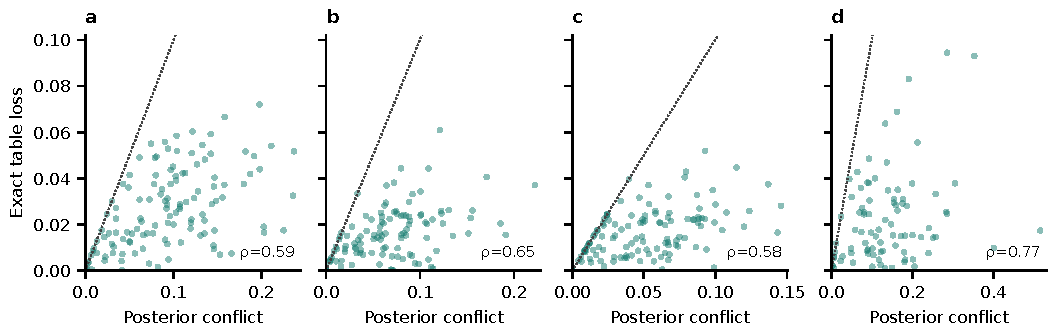
\includegraphics[width=\linewidth]{supplementary/figures/sfig1.pdf}
\caption{Exact labelled-table comparisons at 16 users and 10 dB. Panels a--d show CDL-A, CDL-B, CDL-C and UMa, respectively. Each panel shows 128 independent native blocks. Both axes are in bit/s/Hz. The vertical value is \(R_\beta-D(H)\), and the horizontal value is \(R_\beta-A_\beta\). The dotted diagonal is equality, and each annotation reports its within-profile Spearman correlation. The comparison concerns the rounded integer table.}\label{supp:fig4}
\end{figure}
\begin{figure}[htbp]\centering
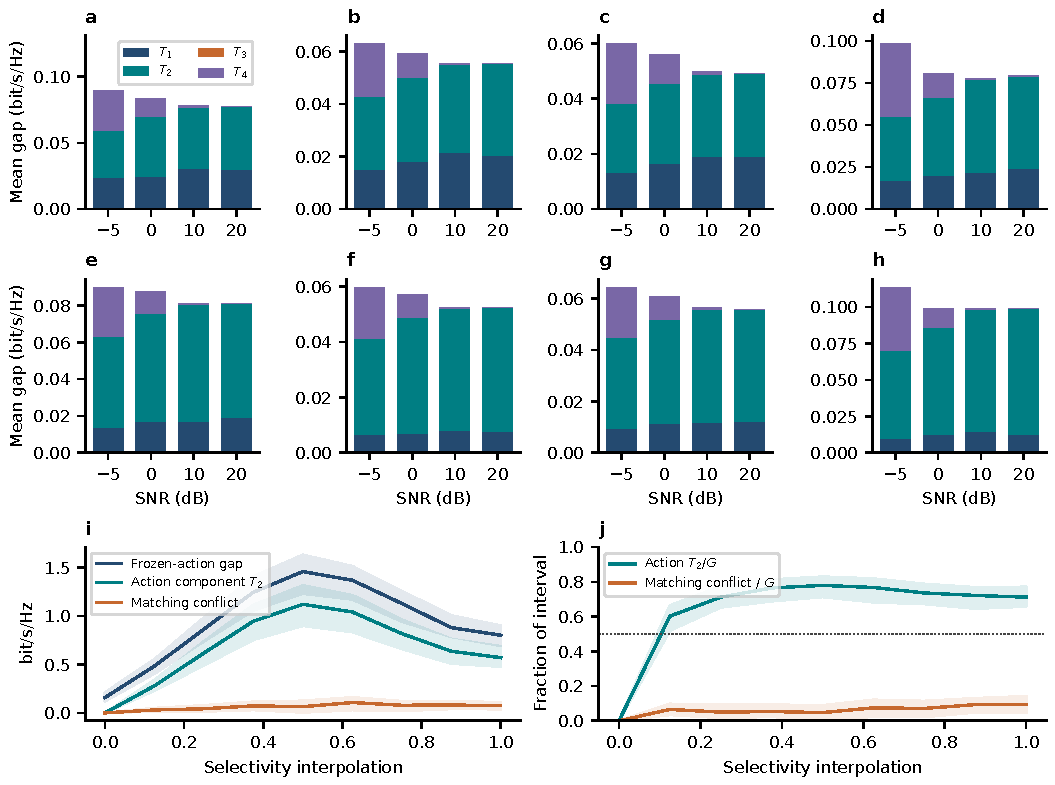
\includegraphics[width=\linewidth]{supplementary/figures/sfig2.pdf}
\caption{Four-term decomposition and the fixed-policy selectivity test. Panels a--d show 32 users and e--h show 64 users, with CDL-A, CDL-B, CDL-C and UMa from left to right. Panels i and j show absolute and relative contributions for the fixed sequential action at 16 users. The upper eight panels stack mean terms over 128 native blocks per profile, size and SNR in the separately timed sensitivity grid. All four means sum to the mean interval, including the small unused-power term. The lower panels show medians and interquartile bands over 128 analytic 16-user blocks at each interpolation. The sequential action's \(T_2\) and the price-selected matching's conflict statistic use different pairings. The dotted line marks one half of the action interval.}\label{supp:fig3}
\end{figure}
\begin{figure}[htbp]\centering
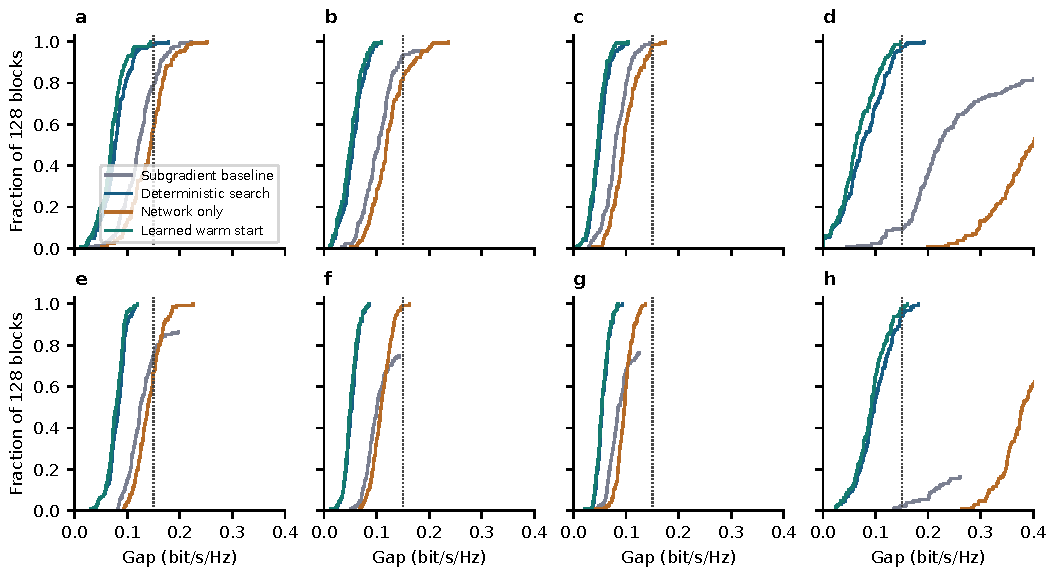
\includegraphics[width=\linewidth]{supplementary/figures/sfig3.pdf}
\caption{Deadline-aware empirical gap distributions within each native profile. Panels a--d show 32 users and e--h show 64 users; within each row the profiles are CDL-A, CDL-B, CDL-C and UMa. Each panel contains 128 independent blocks. Only on-time outcomes increment the curve, and the denominator remains 128. The vertical line is the 0.15-bit/s/Hz criterion. The horizontal display ends at 0.4 bit/s/Hz and retains the full denominator for larger gaps.}\label{supp:fig1}
\end{figure}
\begin{figure}[htbp]\centering
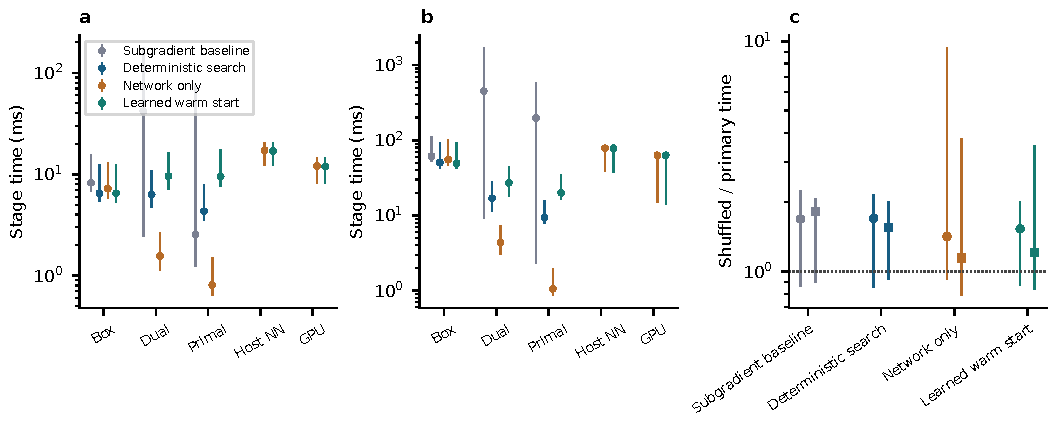
\includegraphics[width=\linewidth]{supplementary/figures/sfig4.pdf}
\caption{Stage-time and load sensitivity. Panels a and b show 32 and 64 users, respectively; panel c shows the shuffled-order comparison. Left and centre, dots show medians and whiskers show p05--p95 across 512 block-level stage medians. Zero GPU/host-network times for the classical methods are omitted on the log axis. GPU and host neural intervals overlap. Right, p05/median/p95 of shuffled-call latency divided by the same block's original median, for 52 blocks. Circles denote 32 users and squares 64 users. Colours identify the same methods throughout.}\label{supp:fig2}
\end{figure}

\FloatBarrier
\section{Propagation geometry and calibration cost}
\label{supp:note5}

\subsection*{Ray-traced channels and the unit of comparison}
The O1\_60 street and ASU Campus 1 scenes provide two propagation geometries from the DeepMIMO collection~\cite{deepmimo}. Each uses base station 1 and 64 disjoint guarded test tiles. The source carrier frequencies are 60 and 3.5 GHz. The tile widths are approximately 1.20 and 12 m, respectively. Thus the comparison combines carrier, propagation geometry and spatial sampling. The same frozen tile supplies nested sets of \(K=16,32,64\) users. Its \(S=K/2\) tones are evenly spaced crops of the original 64-tone, 20-MHz channel. The block scaling used in the archived 10-dB run is applied before computing rates, so the diagnostic follows exactly the normalization of the reported schedule.

Let \(h_{is}\) denote the resulting whitened channel and \(u_{is}=h_{is}/\|h_{is}\|\). On each tone we form the Gram matrix \(Q_s\), whose entries are \(u_{is}^{H}u_{js}\). The two spatial summaries are
\begin{align}
r_{\rm tile}&=\frac{1}{S{K\choose2}}\sum_s\sum_{i<j}|u_{is}^{H}u_{js}|^2,\\
d_{\rm tile}&=\frac1S\sum_s\exp\left(-\sum_\ell t_{\ell s}\ln t_{\ell s}\right),
\qquad t_{\ell s}=\frac{\lambda_\ell(Q_s)}{\operatorname{tr}Q_s},
\end{align}
with \(0\ln0=0\). The effective rank is one for perfectly parallel channels. Its upper bound is the smaller of \(K\) and the 16 receive dimensions. The implementation computes the equal nonzero eigenvalues of the antenna Gram matrix to avoid an unnecessarily large eigendecomposition.

To separate partner choice from power adaptation, fix every user's power at \(p=0.10\) W. For a candidate partner \(j\), the recomputed linear-MMSE rate is
\begin{equation}
R_{i|j,s}=\log_2\left[1+p\|h_{is}\|^2
\left(1-\frac{p\|h_{js}\|^2|u_{is}^{H}u_{js}|^2}
{1+p\|h_{js}\|^2}\right)\right].
\end{equation}
For each user and tone, take the difference between the 90th and 10th percentiles over its \(K-1\) possible partners, using linear sample-quantile interpolation. Average these differences over users and tones to obtain the tile's partner-rate span. Every candidate comparison satisfies the same individual power rails and total budget.

The path counts and direct-path flags come from the original base-station ray records. For each tile, the path statistic is the median count over its selected users. The scene summary is the median of these 64 tile statistics, which can be nonintegral. The LoS statistic instead counts flagged user links over the whole cohort. The channel construction retains at most 25 rays per link. In this comparison, the 32- and 64-user geometry calculations reproduce the previously archived diagnostics. The 16-user calculation uses the same channel digests, original ray-file hashes and nested user ordering, rather than an independent resampling.

\begin{table}[htbp]
\centering
\caption{Ray geometry and certified-gap components at nominal 10 dB. Each row represents 64 guarded tiles. Geometry and rate entries are medians of tile-level values. LoS entries are counts of flagged user links. All rates, gaps and \(T_j\) entries are in bit/s/Hz. Component medians are computed separately and need not sum to the median gap.}
\label{supp:table6}
\small
\begin{tabular}{llrrrrr}
\hline
Scene & \(K\) & Overlap & Effective rank & Paths & LoS links & Partner span\\
\hline
O1 &16&0.9941&1.0199&3.25&1024/1024&1.0536\\
O1 &32&0.9936&1.0218&3.00&2048/2048&1.3234\\
O1 &64&0.9936&1.0230&3.00&4096/4096&1.4779\\
ASU &16&0.4790&2.4907&10.00&116/1024&1.8934\\
ASU &32&0.4649&2.6004&10.00&233/2048&1.9684\\
ASU &64&0.4578&2.6444&10.00&479/4096&2.0964\\
\hline
\end{tabular}

\medskip
\begin{tabular}{llrrrrr}
\hline
Scene & \(K\) & Gap & \(T_1\) & \(T_2\) & \(T_3\) & \(T_4\)\\
\hline
O1 &16&1.1097&0.0000&0.0036&\(6.8793\times10^{-7}\)&1.0929\\
O1 &32&1.1196&0.0004&0.0052&\(6.8793\times10^{-7}\)&1.1133\\
O1 &64&1.0956&0.0002&0.0129&\(6.8793\times10^{-7}\)&1.0713\\
ASU &16&0.0875&0.0232&0.0343&\(6.8793\times10^{-7}\)&0.0093\\
ASU &32&0.1016&0.0199&0.0479&\(6.8793\times10^{-7}\)&0.0074\\
ASU &64&0.0950&0.0137&0.0564&\(6.8793\times10^{-7}\)&0.0053\\
\hline
\end{tabular}
\end{table}

\input{reviewer_refinement}

\subsection*{Reading the decomposition alongside the geometry}
The integer power scale is \(P_T=20\cdot2^{20}\). Projection rounds each scaled excess power down by less than one tick, leaving a small deterministic unused-power charge when the sum budget is active; the repeated median \(T_3=6.8793\times10^{-7}\) bit/s/Hz reflects these power ticks. The four normalized terms retain the definitions of Supplementary Note~2. \(T_1\) measures slack between the certified matching upper and the chosen partners' priced scores, \(T_2\) measures the cost of assigning distinct tones to those partners, \(T_3\) prices unused power, and \(T_4\) compares local continuous-power upper scores with the achieved-action lower rate. The sum is checked against the stored gap for all 384 tile--size records. At each size \(T_4\) has the largest component median on O1, while \(T_2\) has the largest component median on ASU. In particular, at 32 users ASU's \(T_2=0.0479\) exceeds its \(T_1=0.0199\), \(T_4=0.0074\) and \(T_3=6.8793\times10^{-7}\).

O1's nearly unit overlap and effective rank close to one indicate little spatial discrimination between users. Direct and reflected rays can reinforce nearly aligned array responses even when several physical paths are present. This helps interpret the large local rate interval on O1. The fixed-power partner span is nevertheless smaller there than on ASU at all three sizes. A large \(T_4\) therefore quantifies looseness between a local upper calculation and a particular achieved lower rate, rather than measuring sensitivity of user rate to partner choice. Figure~\ref{supp:fig5} displays the distributions underlying the summaries.

\begin{figure}[htbp]
\centering
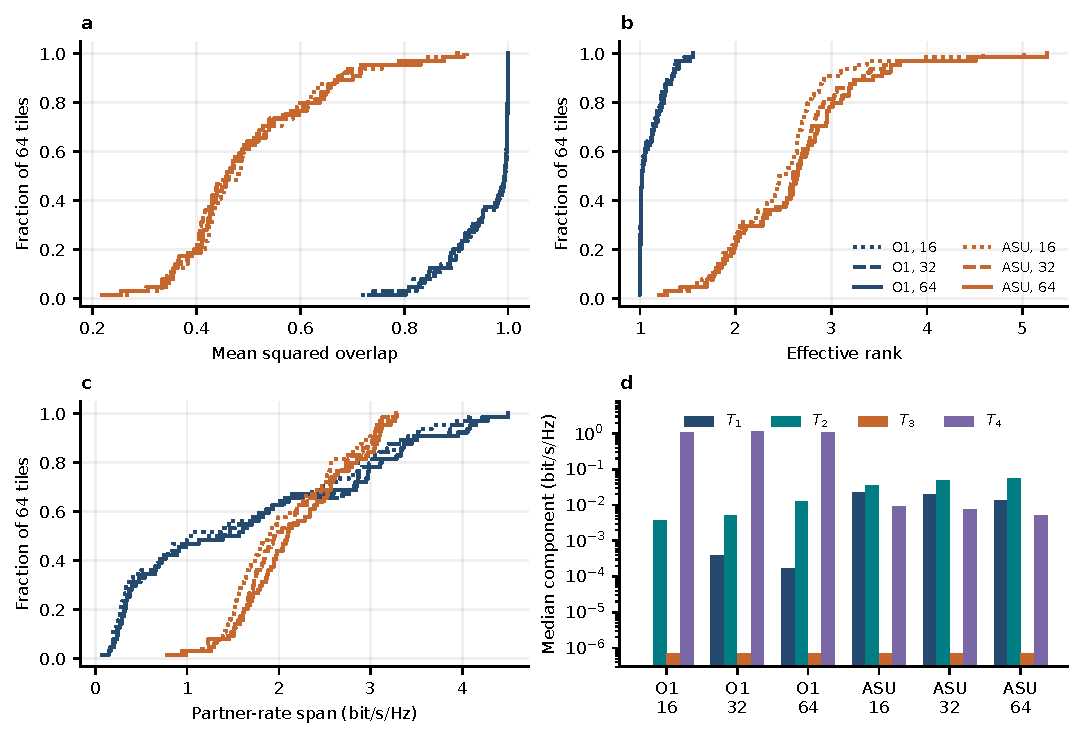
\includegraphics[width=\textwidth]{supplementary/figures/sfig5.pdf}
\caption{Propagation geometry and the four-term decomposition. \textbf{a--c}, Empirical cumulative distributions across 64 guarded tiles per scene and size. Colour identifies the scene, and dotted, dashed and solid curves identify 16, 32 and 64 users. The overlap, effective rank and fixed-power partner span are calculated as defined in this note. \textbf{d}, Separately calculated medians of the four normalized gap components on a logarithmic scale. A zero \(T_1\) median for 16-user O1 has no positive height on this scale. No uncertainty bars are plotted.}
\label{supp:fig5}
\end{figure}

\subsection*{Charging for pilots over a stationary horizon}
The net-gain experiment evaluates two fixed feasible actions on the same least-squares channel estimate, the zero-price, equal-power-initialized matching control with feasible power refinement \(c\) and a learned-initialized action \(w\). The rate intervals \([l_c,u_c]\) and \([l_w,u_w]\) use the stored powers, pairs and receive filters. Four calibration events, two per policy, share a total error probability of 0.05. Each uses rank \(\lceil257(1-0.0125)\rceil=254\) among 256 independent calibration blocks.

A block contains 256 symbols with 32 routine pilot symbols. Charging the warm action for \(M\) additional 32-symbol reference blocks over \(N_{\rm blk}\) stationary blocks gives
\begin{equation}
\eta_c=1-\frac{32}{256},\qquad
\eta_w=\max\left(0,\eta_c-\frac{32M}{256N_{\rm blk}}\right),
\end{equation}
and the budget is affordable if \(32M+32N_{\rm blk}\leq256N_{\rm blk}\). The net-rate interval is
\begin{equation}
[\eta_w l_w-\eta_c u_c,\ \eta_w u_w-\eta_c l_c].
\end{equation}
A positive outcome requires affordability and a lower endpoint above \(10^{-5}\) bit/s/Hz. A negative outcome requires affordability and an upper endpoint below \(-10^{-5}\). The remaining affordable cases are indeterminate. The evaluated horizons are \(1,4,16,64,256,1024\), and extra pilot-block counts are \(0,16,64,256,1024\). Each of the four channel/energy arms contains 128 held-out topologies. Holding the rates fixed makes the \(M=0\) fraction independent of \(N_{\rm blk}\). Transporting this calculation to a changing future channel sequence would require uncertainty calibration over that sequence.

\input{reviewer_horizon}

\begin{figure}[htbp]\centering
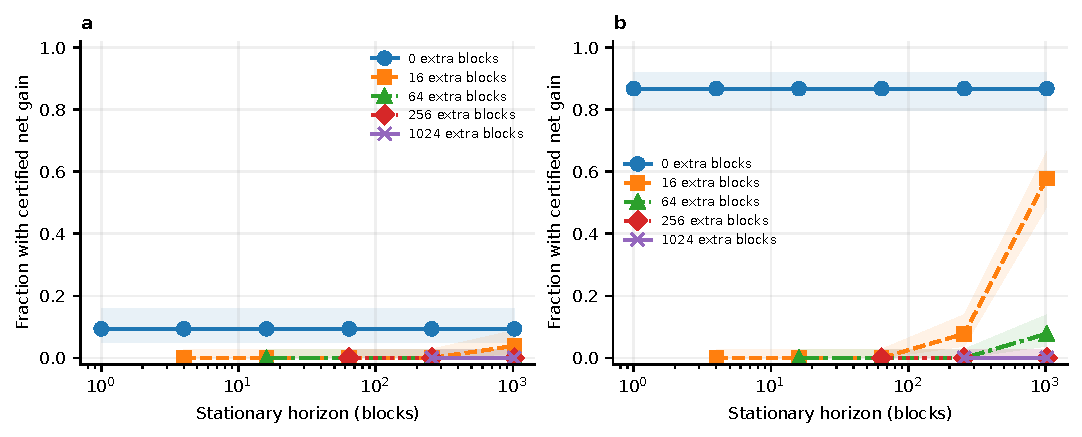
\includegraphics[width=\textwidth]{supplementary/figures/sfig6.pdf}
\caption{Stationary net-rate accounting. Fractions with a certified positive net advantage are shown against the number of stationary blocks for fixed and scaled pilot energy. Curves identify additional pilot-block charges. Only affordable points are drawn. Shaded bands are exact two-sided 95\% binomial intervals over 128 independent simulated topologies; they do not describe uncertainty about an unobserved future time series.}\label{supp:fig6}
\end{figure}

\FloatBarrier
\clearpage
\section{Hardware measurement processing}
\label{supp:note6}

\subsection*{Rice RENEW acquisition, frequency conventions and calibration}
The RENEW analysis uses the registered Rice distributed multi-user MIMO collection.
Each listed file contains 2,001 frame slots, six time-orthogonal client pilot slots,
64 stored receive-stream slots and a noise slot. The selected distributed chain-A
recordings are \texttt{trace-uplink-2022-11-14-2-42-48\_1\_64x6\_0\_63\_chA.hdf5}
(HUB) and \texttt{trace-uplink-2022-11-14-7-10-53\_1\_64x6\_0\_63\_chA.hdf5}
(LO). The carrier is 3.6 GHz and the sample rate is 5 MHz, giving 78.125 kHz
spacing for a 64-point FFT. We retain the recorded ADC scale. Diagonal noise
normalization supplies the receiver's noise metric in these units.

Let $x_{fuan}$ denote the complex ADC sample at time $n$, frame $f$, user $u$
and receive stream $a$. Interleaved signed integers are converted by
$x=(I+\mathrm{i}Q)/32768$. The recorded time-domain pilot and frequency-domain
pilot determine whether the frequency array has been FFT-shifted. For signed
frequency $q\in\{-32,\ldots,31\}$ the two zero-based storage conventions are
\begin{equation}
 b_{\rm centred}(q)=q+32,\qquad b_{\rm native}(q)=q\bmod64.
\end{equation}
Sorting the 48 data tones by signed frequency and taking positions 12, 24 and
36 selects $q=(-13,1,14)$. These map to $(19,33,46)$ in the distributed files
and $(51,1,14)$ in the unshifted colocated LoS files. The four control-pilot
tones and DC are excluded. The decoder explicitly checks the recorded pilot
against both FFT conventions before selecting tones.

The nominal FFT windows are $[176,240)$ and $[256,320)$ within each
1,120-complex-sample slot, with prefix 160 and cyclic prefix 16.
For repetition $r\in\{0,1\}$, with $t_r=176+80r$, the channel estimate is
\begin{equation}
 \widehat h^{(r)}_{fua}(q)=\frac{1}{P(q)}
 \sum_{n=0}^{63}x_{fua,t_r+\ell_u+n}e^{-2\pi\mathrm{i}qn/64},
 \label{supp:eq_renew_fft}
\end{equation}
where $P(q)$ is the recorded pilot and $\ell_u$ is the frozen per-user timing
correction. Calibration scans even shifts from $-64$ to $64$, maximizing
the median log occupied-to-null FFT-energy ratio over reserved frames and
streams, using repetitions indexed 1 through 8. Equal scores prefer the
smallest absolute shift. HUB shifts are $(0,-6,-6,-8,-4,-2)$ samples and LO
shifts are $(-12,-10,-10,-16,-10,64)$. The same shift applies to both windows,
which remain disjoint. The LO sixth-user shift reaches the search boundary,
an observable limitation of this alignment rule.

Frames 0--127 form a reserved calibration prefix. Quality checks use frames
$32,40,\ldots,120$ whose minimum six-user aggregate pilot/noise power ratio
exceeds two. Synchronization uses the first four surviving frames. A receive
stream is retained when at least one user has pilot/noise power at least
6 dB and mean normalized adjacent-LTS coherence at least 0.60, computed
from repetitions 2 through 7 in those calibration frames. This selects
64 HUB and 63 LO streams. The per-stream, per-tone variance is frozen as
\begin{equation}
 \widehat\sigma_a^2(q)=\frac{1}{256}\sum_{f=0}^{127}\sum_{r=0}^{1}
 \left|\mathcal F_{64}\{x^{\rm noise}_{fa,t_r:t_r+64}\}(q)\right|^2,
 \qquad h^{(r)}_{fua}(q)=\widehat h^{(r)}_{fua}(q)/\widehat\sigma_a(q).
\end{equation}
The noise windows use nominal offsets. This is diagonal variance calibration
and carries neither an estimate of cross-stream noise covariance nor a
calibration of radiated transmit power.

\clearpage
\subsection*{RENEW replay, exclusions and mirrored-directory evidence}
For each post-prefix frame, all six pilots must be present, all retained
streams must contain nonzero pilot samples and the extracted noise powers
must be positive. Each user's median retained-stream decision-window to
preceding-guard power ratio must be at least two. Every failed frame remains
in the denominator of 1,873. The early LTS determines the schedule, powers,
filters and recorded-input interval. The identical action is evaluated on
the later LTS as a reference proxy. Its median difference from the early
lower endpoint is $-2.501$ (HUB) and $-4.873$ (LO) bit/s/Hz. All retained
later references fall below that endpoint. This discrepancy limits temporal
interpretation of the early-input certificate.

\begin{table}[htbp]
\centering\small
\caption{RENEW full-capture and nested-window results. A useful decision has
$G\leq0.10$ bit/s/Hz and elapsed time $\leq250$ ms. Nested entries list
$K=2,4,6$ in that order and give medians over 32 accepted windows per listed
stratum. Source-directory labels are preserved.}
\label{supp:table8}
\begin{tabular}{lrrrrr}
\hline
Full chain-A capture & RF & Retained/1,873 & Useful/1,873 & Median $G$ & Median ms\\
\hline
Distributed HUB LoS &64&1,870&1,867&0.00005190&2.7548\\
Distributed LO LoS &63&1,769&1,037&0.07479139&2.7082\\
\hline
\multicolumn{6}{l}{Nested sensitivity, 32 windows per $K$}\\
Directory and chain & RF & \multicolumn{3}{c}{Median $G$ for $K=2,4,6$} & Useful\\
\hline
Colocated HUB LoS A &63&0.0003919&0.00004754&0.00004195&32/32 each\\
Colocated HUB LoS B &63&0.0005810&0.00004160&0.00374474&32/32 each\\
Colocated HUB NLoS A &64&0.0003452&0.00007622&0.00006767&32/32 each\\
Colocated HUB NLoS B &64&0.0005105&0.00004837&0.00007956&32/32 each\\
Distributed HUB LoS A &64&0.0003452&0.00007622&0.00006767&32/32 each\\
Distributed HUB LoS B &64&0.0005105&0.00004837&0.00007956&32/32 each\\
Distributed LO LoS A &63&0.0015542&0.00016973&0.00012370&32/32 each\\
\hline
\end{tabular}
\end{table}
\subsection*{Chronological directional calibration and exhaustive pairing}
The first 128 frames continue to determine timing, RF selection and noise variance only. Among the eligible post-prefix frames, the first 256 form a new chronological calibration set and the remainder form a disjoint test set. The scheduling map takes only the early pilot. For frame $f$, let $\Delta h_{fus}=h^{(1)}_{fus}-h^{(0)}_{fus}$ and let $\bar v_{fis}$ be the unit-normalized early-input filter. We use scalar whole-frame scores
\[
 s_{F,f}=\max_{u,s}\|\Delta h_{fus}\|_2,\qquad
 s_{P,f}=\max_{(i,j,s)\text{ scheduled}}\max_{k\in\{i,j\}}
 |\bar v_{fis}^{H}\Delta h_{fks}|.
\]
Both receiver directions in each pair are included. The 251st sorted score of 256 calibration frames, rounded outward, supplies each radius. The same projected radius is used for every desired/interference projection within a frame. Vector and projected events each receive error budget 0.025. The test has 1,614 HUB and 1,513 LO frames. Every lower and upper certificate is replayed by the separate numerical checker. Empirical floor coverage counts $R_{\rm later}\geq L_P$; interval coverage uses $\max(L_P,L_F)\leq R_{\rm later}\leq U_F$. The reported projected width is $U_F-L_P$.

These residuals include pilot noise, synchronization differences and channel evolution. No component is identified separately. The temporal split avoids reusing calibration residuals for testing, but successive frames are not independent replicates. We therefore do not use the conformal rank formula as evidence of population coverage, or attach an independent-binomial confidence interval to these recording-level fractions. All coverage statements concern the second observable LTS and the stored early-input action.

At six users and three labelled tones, sorting the two user indices within each pair leaves $6!/2^3=90$ schedules. We enumerate all 90 with fixed powers of 0.10 and the MMSE pair rate on the early input. This is exhaustive over the stated discrete set; the rates are floating-point numerical evaluations. Its optimum is a feasible reference for the continuous-power model, not that model's exact optimum.


\subsection*{Phase-invariant scores and the thermal-noise benchmark}
For each user and frame we calculate the phase of the inner product of the early and later channel vectors concatenated over all retained streams and three tones. Over test user--frame pairs, median absolute rotations are 0.041899 rad on HUB (IQR 0.019987--0.071188) and 0.259930 rad on LO (0.233082--0.286302). Dividing by \(2\pi(16~\mu{\rm s})\) gives equivalent absolute frequency offsets of 0.416773 kHz (0.198816--0.708123) and 2.585568 kHz (2.318505--2.847896). These conversions attribute the entire phase change to frequency offset for scale; the replay does not identify a causal oscillator model.

For the projected magnitude score and phase-aligned vector score, respectively, we use
\[
s^{\rm mag}_{P,f}=\max_{(i,j,s),\,k\in\{i,j\}}
\left||\bar v_{fis}^Hh^{(1)}_{fks}|-|\bar v_{fis}^Hh^{(0)}_{fks}|\right|,
\qquad
s^{\rm ph}_{F,f}=\max_{u,s}\min_\theta
\|e^{-{\rm i}\theta}h^{(1)}_{fus}-h^{(0)}_{fus}\|_2 .
\]
The vector alignment minimizes separately for each user/tone; the diagnostic phase above is instead one concatenated phase per user/frame. Both scores retain the original 256 calibration frames, rank 251 and test frames. If a magnitude residual is at most \(b_{ik}\), the desired amplitude is bounded below by \((|\bar v_i^Hh_i^{(0)}|-b_{ii})_+\), and the interfering amplitude above by \(|\bar v_i^Hh_j^{(0)}|+b_{ij}\). The SINR is increasing in the first squared amplitude and decreasing in the second, proving the projected floor conditionally on those bounds; the vector oracle is unchanged by user/tone phase rotations. The implementation checks rate/score phase invariance and replays every numerical certificate.

As a thermal-noise-only benchmark, independently drawn proper complex pilot errors of unit variance give difference variance two. A unit-filter projection then has tail probability \(\exp(-x^2/2)\); a union bound over 12 projections gives the 97.5\% threshold \(\sqrt{2\log(12/0.025)}=3.51391\). The expected maximum for 12 independent projections is 2.44453. Holding the observed early filters fixed and retaining correlations between projections, 16,384 Monte Carlo blocks per capture give expected maxima 2.44987 (HUB) and 2.44705 (LO), with Monte Carlo standard errors 0.00377 and 0.00378. This benchmark isolates noise and does not model the dependence of estimated filters on their noisy pilots, cross-stream noise correlation, or drift. The observed raw radii of 87.36 and 165.26 greatly exceed it. Removing phase sensitivity raises the floors, yet LO joint-event coverage remains 75.74\%, below nominal 95\%; its universal floor coverage is sustained by slack.

\input{reviewer_hardware}


The sensitivity replay selects 32 integer-spaced frames from 128 to 1,999,
with users $1{:}K$ and tone sets $\{1\}$, $\{-13,14\}$ and $\{-13,1,14\}$
for $K=2,4,6$. Thus the user subsets are nested and each replay has $K/2$
tones. Its calibration uses candidate prefix frames $(32,56,80,104)$,
retaining the pilot-present subset for noise estimation and quality masking.
These smaller-prefix estimates explain why its gaps differ from the
full-capture replay. LO chain B failed calibration and contributes no window.

\begin{figure}[htbp]
\centering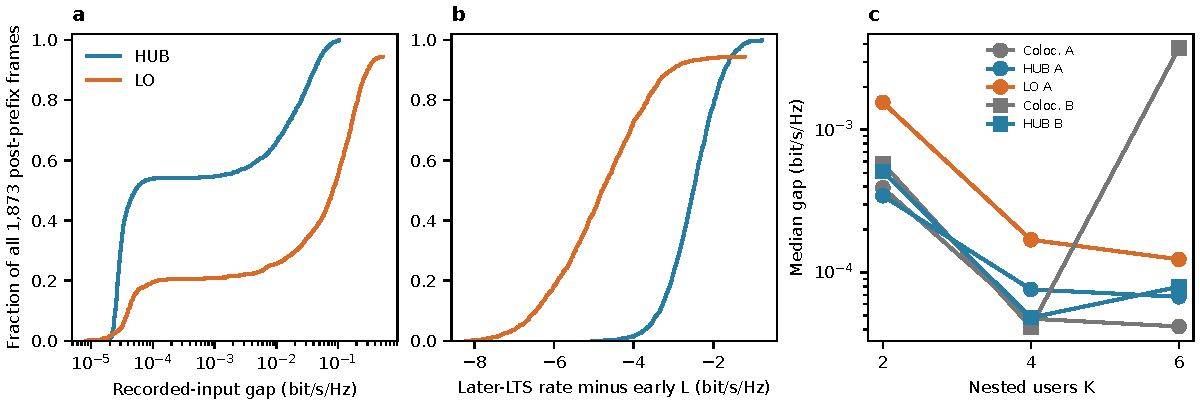
\includegraphics[width=\linewidth]{supplementary/figures/sfig7.pdf}
\caption{RENEW recorded-input gap distributions (a), later-LTS fixed-action
rate minus early lower endpoint (b), and nested-window sensitivity (c).
Both ECDFs use all 1,873 post-prefix frames per mode as their denominator,
so their final heights expose abstentions. Panel c omits the mirrored NLoS
directory curves, which coincide with the distributed HUB curves.}
\label{supp:fig7}
\end{figure}

\clearpage
\subsection*{Provenance and acquisition scope}
The colocated HUB NLoS and distributed HUB LoS directory entries have matching
filenames, lengths and acquisition timestamps. Independently requested common
byte ranges have matching SHA-256 digests for 24/24 chain-A ranges and 22/22
chain-B ranges. Sampled pilot and noise arrays also match. The evidence
supports probable directory mirroring. Physical placement remains dependent
on source-side provenance. These entries therefore add no independent
replication. Full-capture SHA-256 digests are
\begin{quote}\footnotesize\ttfamily
HUB\quad\nolinkurl{aec556198de39208757fddc294af77d4f701d7a24b9f1feb3f1fdc09d36bc0d2}\\
LO\quad\nolinkurl{e5fabc009dce96e527b6919ce744f0b41408f337e0d5334b8dadfa0f13699844}.
\end{quote}
Each distributed clock mode supplies one acquisition. Frames, user subsets,
RF chains and tones are repeated observations within this evidence base.
The six-user offline scheduling counterfactual has no measured counterfactual
payload throughput. The two disjoint LTS windows provide a temporal proxy
comparison with an empirically substantial discrepancy. Hardware population
coverage and a causal clock-mode comparison require additional acquisitions.

The separate CPU implementation reconstructed the full RENEW distributions from archived accepted-frame
and abstention records. Its authenticated source spot check fetched frame 128
and calibration-noise frames $(56,80,104)$ for HUB and $(80,104)$ for LO,
verifying respectively 18 and 14 source pages. Recomputed mean pair overlaps
were 0.08521393847151353 and 0.06809478943705848, agreeing with archived values
to floating-point precision. Complete distributed IQ captures were unavailable
to that audit. The present supplement regenerates the full distributions from
those archived derived rows and verifies their counts.

\subsection*{Rice Argos six-user correlation statistic and quality masks}
The three Argos UHF recordings are the 28 November 2015 static (14:39:47),
environmental-mobility (14:43:08) and mobile (14:47:06) acquisitions. They contain
12,017, 12,014 and 12,018 frames respectively, six user slots and a seventh
noise slot, recorded through eight RF streams. The analysis protocol reserves
frames 0--63 for RF qualification and fixes 32 interior evaluation frames as
\begin{equation}
 f_j=64+\left\lfloor\frac{(2j+1)(n_f-64)}{64}\right\rfloor,
 \qquad j=0,\ldots,31.
\end{equation}
Each RF record reshapes into seven slots of 224 complex samples. The two
64-sample LTS windows start at zero-based offsets 47 and 111. After a centred
FFT, occupied bins are $6{:}31$ and $33{:}58$, equivalently signed tones
$-26{:}-1$ and $1{:}26$. The remaining 12 bins contain DC and guard tones.
The seventh slot is excluded from user-pair statistics.

Let $H^{(r)}_{fua}(q)$ be the resulting occupied-bin vector. The quality
measure divides mean occupied-bin energy by mean null-bin energy, averaging
both LTS windows. Adjacent-LTS coherence is the magnitude of their tonewise
inner product divided by the product of their norms. An RF stream is
qualified if at least one user has median calibration concentration at least
6 dB and median coherence at least 0.60. All eight streams qualify in every
recording. An evaluation frame must supply all six finite, nonzero channel
vectors on all 52 tones, at least two qualified streams, and for every user
median concentration at least 3 dB and median coherence at least 0.50 over
retained streams. Failed frames are retained as abstentions and never replaced.

\clearpage
For unordered pair $(u,v)$, define
\begin{equation}
 \rho^{(r)}_{fuv}(q)=
 \frac{|(H^{(r)}_{fu}(q))^{\!H}H^{(r)}_{fv}(q)|^2}
 {\|H^{(r)}_{fu}(q)\|^2\|H^{(r)}_{fv}(q)\|^2},\quad
 c^{(r)}_{fuv}=\frac1{52}\sum_q\rho^{(r)}_{fuv}(q),\quad
 \bar c^{(r)}_f=\frac1{15}\sum_{u<v}c^{(r)}_{fuv}.
\end{equation}
Supplementary Table~\ref{supp:table9} gives medians and quartiles of $\bar c^{(r)}_f$ over
qualified frames, with paired changes calculated before taking the median.
Supplementary Fig.~\ref{supp:fig8} instead gives the median of each pair's
$c^{(r)}_{fuv}$ over those same frames. Their different aggregation orders
are explicit. The heatmaps are recomputed from locally retained IQ windows,
with all 99 source-range digests and three frame-zero digests checked. Every
recomputed pair/frame mean agrees with the archived scalar statistic to
absolute tolerance $2\times10^{-13}$ plus relative tolerance $10^{-12}$.
Controls cover orthogonal, identical, zero and phase-rescaled vectors.

\begin{table}[htbp]
\centering\small
\caption{Argos first- and second-LTS spatial correlations. Brackets are
within-recording first and third quartiles. The unfiltered column includes
all 32 finite planned frames. All values are dimensionless.}
\label{supp:table9}
\begin{tabular}{lrrrrr}
\hline
Recording & Retained & First LTS & Second LTS & Paired change & Unfiltered first\\
\hline
Static &31/32&0.2250&0.2378&0.0176&0.2224\\
 & &[0.2051,0.2405]&[0.2230,0.2498]&[-0.0036,0.0305]&\\
Environmental &32/32&0.2402&0.2533&0.0083&0.2402\\
 & &[0.2250,0.2533]&[0.2387,0.2614]&[0.0003,0.0215]&\\
Mobile &22/32&0.2250&0.2430&0.0108&0.2288\\
 & &[0.2158,0.2356]&[0.2302,0.2514]&[0.0033,0.0304]&\\
\hline
\end{tabular}
\end{table}
\begin{figure}[htbp]
\centering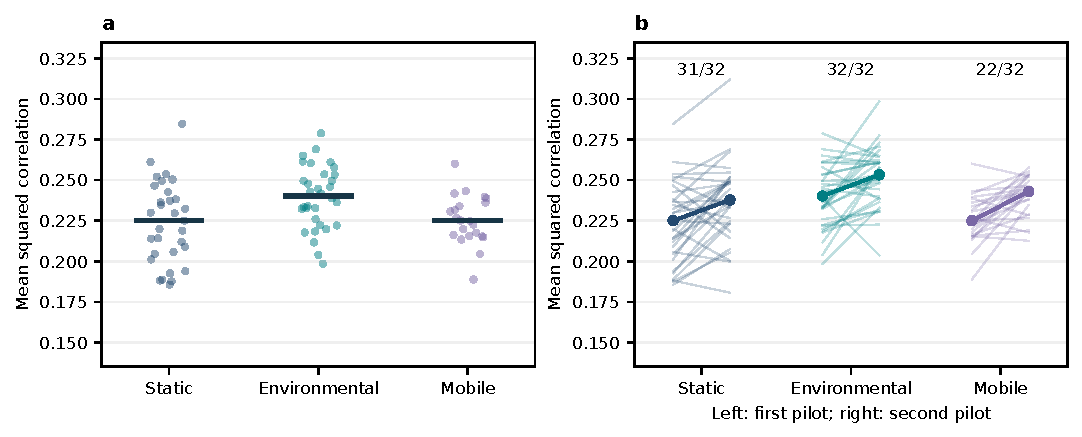
\includegraphics[width=0.92\linewidth]{supplementary/figures/sfig8.pdf}
\caption{Argos spatial overlap on two recorded pilots. \textbf{a}, First-LTS mean squared correlation on each qualified frame, with horizontal segments marking medians. \textbf{b}, Thin lines join the first and second LTS from the same frame; thick lines join the medians. Counts give qualified frames out of 32 planned frames. Both repetitions use identical RF masks. These panels describe spatial separation, not paired-payload throughput.}
\label{supp:fig8}
\end{figure}
The three recordings describe one array setup with one recording per
condition. Their spatial correlations support a small-load hardware
description. Supplementary data contain derived scalar summaries and hashes.
Access to the original IQ and reconstructed complex channels follows Rice's research-use terms.


Platform credit belongs to the Rice RENEW team and M. Zafari's distributed
multi-user MIMO dataset (doi:10.21227/74ez-b275), and to C. Shepard,
J. Ding, R. E. Guerra and L. Zhong, \emph{Understanding Real Many-Antenna
MU-MIMO Channels} (Asilomar 2016), for the Argos recordings.

\FloatBarrier
\section{Outward channel bounds and integer matching verification}
\label{supp:note3}

\paragraph{Channel grid and exact Gram products.}
Let \(h\in\mathbb C^{K\times N\times S}\) be the supplied channel array. The integrated implementation accepts \(2\leq K\leq64\), \(K=2S\), \(1\leq N\leq256\), nonnegative finite radii, and a largest absolute real or imaginary component between \(2^{-100}\) and \(2^{100}\). Choose a common power-of-two spacing \(\delta\) so that nearest-integer rounding of each component divided by \(\delta\) has magnitude at most \(2^{22}\). For integer vectors \(a_i,b_i\) representing real and imaginary parts, the centre Gram entries are
\begin{equation}
 \widetilde h_i^H\widetilde h_j
 =\delta^2\left[
    a_i^\mathsf T a_j+b_i^\mathsf T b_j
    +\mathrm i(a_i^\mathsf T b_j-b_i^\mathsf T a_j)\right].
\end{equation}
Each bracketed real component sums at most \(2N\) products of magnitude \(2^{44}\). Thus its absolute value and the sum of absolute intermediate products are at most
\(2N2^{44}\leq2^{53}\). Integer accumulation and power-of-two rescaling preserve these sums exactly within the supported range. If the input channel has radius \(\epsilon_i\), the rounded centre receives the outward radius
\begin{equation}
 \widetilde\epsilon_i\geq\epsilon_i+\frac{\delta\sqrt{2N}}{2}.
\end{equation}
This covers the worst-case displacement of all \(2N\) real coordinates.

For centres \(a,b\) and padded radii \(u,v\), expanding the inner product and applying Cauchy--Schwarz gives
\begin{equation}
 |h_i^Hh_j|\geq
 \left[|a^Hb|-\|a\|v-\|b\|u-uv\right]_+ .
\end{equation}
Squaring this lower bound and dividing by upper squared channel norms produces a lower squared normalized overlap. Norm bounds also give lower and upper received gains. For
\(\gamma(x,y,r)=x(1-r y/(1+y))\), with \(x,y\geq0\) and \(0\leq r\leq1\), monotonicity is increasing in \(x\) and decreasing in \(y,r\). Evaluating each user's desired term at its upper gain and power, and interference at the lower partner gain, power and overlap, therefore bounds the rate over an entire two-dimensional power box. Subtraction of a lower power charge preserves the upper bound.

\paragraph{Binary64 elementary and logarithmic operations.}
The arithmetic contract uses nearest-even IEEE binary64 operations, gradual underflow and disabled fast-math reassociation. Applying \(\operatorname{nextafter}\) toward \(-\infty\) or \(+\infty\) to a rounded elementary result encloses the corresponding real result. Exceptional values cause rejection or retention of an available valid upper bound. The compiled reference logarithm writes \(x=2^k t\), \(1\leq t<2\), and uses \(z=(t-1)/(t+1)\leq1/3\):
\begin{equation}
 \ln t=2\sum_{j=0}^{19}\frac{z^{2j+1}}{2j+1}+R_{20},
 \qquad
 0\leq R_{20}\leq\frac{2z^{41}}{41(1-z^2)}.
 \label{supp:eq:binarylog}
\end{equation}
Every term and the remainder are enclosed outward. The result is combined with an enclosure of \(k\ln2\), reversing interval endpoints when \(k<0\).

The integrated scheduler reuses this 20-term routine to tabulate 257 outward values of \(\ln(1+j/256)\). For a mantissa \(t\), choose \(a=1+\lfloor256(t-1)\rfloor/256\). Then \(z=(t-a)/(t+a)<1/512\) and
\[
 \ln t=\ln a+2\left(z+\frac{z^3}{3}+\frac{z^5}{5}\right)+R,
 \qquad 0\leq R\leq\frac{2z^7}{7(1-z^2)}.
\]
The runtime implementation bounds the tail conservatively using \(z^7/3\) and outward coefficient allowances. This three-term local evaluation and the 20-term table construction both preserve a complete logarithmic enclosure. The rational Gaussian integration of Supplementary Note~\ref{supp:note2} separately uses its 18-term integer series.

\paragraph{Complete roots and lazy subdivision.}
Each pair--tone entry initially covers the full power square \([p_-,p_+]^2\). A cached unpriced root can be used at several nonnegative power prices by subtracting a lower bound on the charge. Priorities choose entries for optional refinement. Splitting each power interval at four shared subinterval boundaries produces 16 children whose union covers the parent, including boundaries. If \(H_{\mathrm{old}}\) and \(H_c\) are valid upper bounds for the parent and children, respectively, then
\begin{equation}
 H_{\mathrm{new}}=\min\!\left(H_{\mathrm{old}},\max_{c=1,\ldots,16}H_c\right)
 \label{supp:eq:lazyroot}
\end{equation}
remains valid. The parent is retained until every child is covered. This argument also covers incorrect priorities, ties, unselected entries and interrupted optional work. The scheduler additionally uses tangents to the individual concave log terms with a separately enclosed correlation penalty. Every such bound must cover its complete domain before it can tighten an entry.

\begin{table}[htbp]
\centering
\small
\caption{Rate-box evaluation counts in the compiled-kernel fixture. Four candidate power prices use the same cached roots. The optional-leaf and total-call reductions have different denominators. Counts quantify arithmetic work for this fixture; runtime includes additional matching, proposal and verification work.}
\label{supp:table2}
\begin{tabular}{lrr}
\hline
Quantity & \(K=32,\ S=16\) & \(K=64,\ S=32\)\\
\hline
Cached unpriced roots \(M=S\binom K2\) & 7,936 & 64,512\\
Cheap priced-root updates \(4M\) & 31,744 & 258,048\\
Refined entries per price \(b\) & 32 & 128\\
Lazy refinement leaves \(4\cdot16b\) & 2,048 & 8,192\\
Total lazy rate-box calls \(M+64b\) & 9,984 & 72,704\\
Eager leaf calls \(4\cdot16M\) & 507,904 & 4,128,768\\
Eager/lazy optional leaves \(M/b\) & \(248\) & \(504\)\\
Eager/total lazy rate-box calls & \(50.872\) & \(56.789\)\\
\hline
\end{tabular}
\end{table}

\paragraph{Signed integer weights and quarter-tick witness.}
Table entries are rounded upward to the grid \(1/\Gamma\), \(\Gamma=2^{40}\) nats. For any real score, including a negative score,
\(0\leq\lceil\Gamma H\rceil/\Gamma-H<1/\Gamma\). A schedule has \(S\) entries, so its rounding excess is below \(S/\Gamma\). All matching calculations use the same rounded table and integer tone prices.

The C++14 interface requests a maximum-weight \emph{perfect} matching from LEMON 1.3.1. It checks the library's dual scale at compilation and exports the matching, vertex potentials \(Y_i\) and positive odd-set potentials \(Z_B\) in quarter-tick units. The independent checker verifies the exact integer relations
\begin{equation}
 \begin{aligned}
 Y_i+Y_j+\sum_{B:\{i,j\}\subseteq B}Z_B&\geq4w_{ij}
                   &&\text{for every edge},\\
 \sum_iY_i+\sum_B\left\lfloor\frac{|B|}{2}\right\rfloor Z_B
                &=4\sum_{e\in m}w_e,\qquad Z_B\geq0 .
 \end{aligned}
 \label{supp:eq:quartertick}
\end{equation}
It also checks that each user occurs once, each reported set has distinct valid vertices and odd cardinality at least three, and the integer ranges satisfy the implementation limits. The signs of the edge and vertex weights are unrestricted. Summing the first inequalities over any perfect matching and using the odd-set cardinality bound proves the upper bound; equality proves the proposed matching is optimal. A failed witness triggers the checked vertex-price repair. Pair-to-tone assignments are separately verified using feasible row and column potentials with exact objective equality.

The recorded kernel tests include 26 logarithm inputs spanning subnormal and maximum finite values and both sides of one, rational rate-box comparisons, preservation of unrefined roots, and invalid-input and overflow controls. The supplied software includes these numerical checks.

\clearpage
\subsection*{Separate CPU verification and the meaning of its counts}
The separate CPU verification rebuilt verification code in a fresh local environment
and operated on immutable release packages. Independence concerns verification
implementation and execution on the original workstation. Its numerical
specifications share the released enclosure primitives and base mathematical
libraries. The archived results permit independent computational replay of the recorded inputs. Supplementary Table~\ref{supp:table10} separates the
units of evidence so repeated timings, samples and optimization instances
are counted consistently.



The sample protocol ranks units by SHA-256 of the fixed ASCII audit tag,
a zero separator, the binary frozen-input archive digest, another zero separator and
the ASCII source/family/block identity. The 58 smallest hashes are selected
without replacement or outcome filtering. The sample CSV SHA-256 is
\texttt{435d79143ad78221acffb37cea4ed4b7d}\allowbreak\texttt{35144df4476f19f3331ad1c6b40d706}.
The 21/30/7 composition is a result of this hash selection.

For two-user power optimization, with Gram gains $g_1,g_2$ and
$C=g_1g_2-|h_1^Hh_2|^2\geq0$, total power $s=1/5$ and first-user power
$p\in[1/20,3/20]$, the recomputed sum rate is
\begin{equation}
 R(p)=\log\frac{D(p)^2}{E(p)},\quad
 D(p)=1+sg_2+(g_1-g_2+sC)p-Cp^2,\quad
 E(p)=(1+g_1p)(1+g_2(s-p)).
\end{equation}
The derivative has the sign of the rational cubic
$2D'(p)E(p)-D(p)E'(p)$. The audit represents it in the Bernstein basis,
discards intervals whose coefficients certify a common sign, and bisects
ambiguous intervals to depth 90. Boundary points and surviving stationary
candidate boxes are enclosed with exact rational arithmetic and outward
80-digit decimal logarithms. Each of the 512 independent intervals lies
inside its archived global enclosure. The number 512 counts instances,
each of which may have several stationary or boundary candidates.

The seven corruption controls alter, respectively, a sum-preserving transfer
between decomposition terms, the covered-table digest, an odd set, a primal user
assignment by duplication, the sign of a lower-rate tick, the denominator,
and the upward rounding of the displayed gap. Their rejection tests the
specified verifier checks. Hardware-source checks have the distinct scopes
given above. Files \texttt{certificate\_checks.csv}, \texttt{sample\_dp.csv},
\texttt{nested\_small\_dp.csv}, \texttt{exact\_two\_replay.csv} and
\texttt{negative\_controls.json} preserve the corresponding audit evidence.

\input{reviewer_audit}

\clearpage
\renewcommand{\refname}{Supplementary References}
\begin{thebibliography}{51}\small
\bibitem{marzetta} Marzetta, T. L. \href{https://doi.org/10.1109/TWC.2010.092810.091092}{Noncooperative cellular wireless with unlimited numbers of base station antennas}. \emph{IEEE Trans. Wirel. Commun.} \textbf{9}, 3590–3600 (2010).
\bibitem{ngo} Ngo, H. Q., Ashikhmin, A., Yang, H., Larsson, E. G. \& Marzetta, T. L. \href{https://doi.org/10.1109/TWC.2017.2655515}{Cell-free massive MIMO versus small cells}. \emph{IEEE Trans. Wirel. Commun.} \textbf{16}, 1834–1850 (2017).
\bibitem{bjornson} Björnson, E. \& Sanguinetti, L. \href{https://doi.org/10.1109/TWC.2019.2941478}{Making cell-free massive MIMO competitive with MMSE processing and centralized implementation}. \emph{IEEE Trans. Wirel. Commun.} \textbf{19}, 77–90 (2020).
\bibitem{demir} Demir, Ö. T., Björnson, E. \& Sanguinetti, L. \href{https://doi.org/10.1561/2000000109}{Foundations of user-centric cell-free massive MIMO}. \emph{Found. Trends Signal Process.} \textbf{14}, 162–472 (2021).
\bibitem{buzzi} Buzzi, S., D’Andrea, C., Zappone, A. \& D’Elia, C. \href{https://doi.org/10.1109/TWC.2019.2952117}{User-centric 5G cellular networks: resource allocation and comparison with the cell-free massive MIMO approach}. \emph{IEEE Trans. Wirel. Commun.} \textbf{19}, 1250–1264 (2020).
\bibitem{caire} Caire, G. \href{https://doi.org/10.1109/TWC.2018.2808522}{On the ergodic rate lower bounds with applications to massive MIMO}. \emph{IEEE Trans. Wirel. Commun.} \textbf{17}, 3258–3268 (2018).
\bibitem{wang} Wang, Z., Zhang, J., Ngo, H. Q., Ai, B. \& Debbah, M. \href{https://doi.org/10.1109/TCOMM.2023.3235919}{Uplink precoding design for cell-free massive MIMO with iteratively weighted MMSE}. \emph{IEEE Trans. Commun.} \textbf{71}, 1646–1664 (2023).
\bibitem{haustein} Haustein, T. \href{https://edocs.tib.eu/files/e01dd01/522593321.pdf}{Real time signal processing for multi-antenna systems and experimental verification on a reconfigurable hardware test-bed}. \emph{PhD thesis, Technische Universität Berlin} (2006).
\bibitem{viterbo} Viterbo, E. \& Hottinen, A. \href{https://doi.org/10.1109/ISSSTA.2008.50}{Optimal user pairing for multiuser MIMO}. \emph{Proc. 10th IEEE Int. Symp. Spread Spectrum Tech. Appl. (ISSSTA)}, 242–246 (2008).
\bibitem{fan} Fan, J., Li, G. Y., Yin, Q., Peng, B. \& Zhu, X. \href{https://doi.org/10.1109/TWC.2012.070912.111305}{Joint user pairing and resource allocation for LTE uplink transmission}. \emph{IEEE Trans. Wirel. Commun.} \textbf{11}, 2838–2847 (2012).
\bibitem{ruder2013} Ruder, M. A., Ding, D., Dang, U. L., Vasilakos, A. V. \& Gerstacker, W. H. \href{https://doi.org/10.1016/j.phycom.2013.02.004}{Joint user grouping and frequency allocation for multiuser SC-FDMA transmission}. \emph{Phys. Commun.} \textbf{8}, 91–103 (2013).
\bibitem{ruder2014} Ruder, M. A., Moldovan, A. \& Gerstacker, W. H. \href{https://doi.org/10.1016/j.phycom.2014.10.001}{SC-FDMA user pairing and frequency allocation with imperfect channel state information}. \emph{Phys. Commun.} \textbf{13}, 88–98 (2014).
\bibitem{prasad} Prasad, N., Zhang, H., Zhu, H. \& Rangarajan, S. \href{https://doi.org/10.1109/TWC.2013.072513.120734}{Multi-user MIMO scheduling in the fourth generation cellular uplink}. \emph{IEEE Trans. Wirel. Commun.} \textbf{12}, 4272–4285 (2013).
\bibitem{viswanath} Viswanath, P., Tse, D. N. C. \& Anantharam, V. \href{https://doi.org/10.1109/18.904525}{Asymptotically optimal water-filling in vector multiple-access channels}. \emph{IEEE Trans. Inf. Theory} \textbf{47}, 241–267 (2001).
\bibitem{shi} Shi, S., Schubert, M. \& Boche, H. \href{https://doi.org/10.1109/TSP.2008.924796}{Rate optimization for multiuser MIMO systems with linear processing}. \emph{IEEE Trans. Signal Process.} \textbf{56}, 4020–4030 (2008).
\bibitem{shenfpone} Shen, K. \& Yu, W. \href{https://doi.org/10.1109/TSP.2018.2812733}{Fractional programming for communication systems—Part I: Power control and beamforming}. \emph{IEEE Trans. Signal Process.} \textbf{66}, 2616–2630 (2018).
\bibitem{shenfptwo} Shen, K. \& Yu, W. \href{https://doi.org/10.1109/TSP.2018.2812748}{Fractional programming for communication systems—Part II: Uplink scheduling via matching}. \emph{IEEE Trans. Signal Process.} \textbf{66}, 2631–2644 (2018).
\bibitem{sun} Sun, H. et al. \href{https://doi.org/10.1109/TSP.2018.2866382}{Learning to optimize: training deep neural networks for interference management}. \emph{IEEE Trans. Signal Process.} \textbf{66}, 5438–5453 (2018).
\bibitem{shen} Shen, Y., Shi, Y., Zhang, J. \& Letaief, K. B. \href{https://doi.org/10.1109/JSAC.2020.3036965}{Graph neural networks for scalable radio resource management: architecture design and theoretical analysis}. \emph{IEEE J. Sel. Areas Commun.} \textbf{39}, 101–115 (2021).
\bibitem{hejazicluster} Hejazi, P. \& Sabaei, M. \href{https://doi.org/10.23919/JCN.2025.000085}{Optimizing spectral efficiency through user clustering in user-centric cell-free massive MIMO environment for 6G wireless network}. \emph{J. Commun. Netw.} \textbf{28}, 30–39 (2026).
\bibitem{ahmadi2026} Ahmadi, N. \& Akbarizadeh, G. \href{https://doi.org/10.1038/s41598-026-38685-3}{Machine learning based power control in cellular and cell-free massive MIMO systems}. \emph{Sci. Rep.} \textbf{16}, 8129 (2026).
\bibitem{hamakawa2026} Hamakawa, Y., Kashimata, T., Yamasaki, M. \& Tatsumura, K. \href{https://doi.org/10.1038/s41467-026-73725-6}{Machine learning-assisted high-speed combinatorial optimization with Ising machines for dynamically changing problems}. \emph{Nat. Commun.} \textbf{17}, 4877 (2026).
\bibitem{kashimata2026} Kashimata, T., Hamakawa, Y., Yamasaki, M. \& Tatsumura, K. \href{https://doi.org/10.1038/s41467-026-76069-3}{Real-time black-box optimization for dynamic discrete environments using embedded Ising machines}. \emph{Nat. Commun.} \textbf{17}, 8085 (2026).
\bibitem{dinitz} Dinitz, M., Im, S., Lavastida, T., Moseley, B. \& Vassilvitskii, S. \href{https://proceedings.neurips.cc/paper/2021/hash/5616060fb8ae85d93f334e7267307664-Abstract.html}{Faster matchings via learned duals}. \emph{Adv. Neural Inf. Process. Syst.} \textbf{34}, 10393–10406 (2021).
\bibitem{bessa} Bessa, S., Dabert, D., Bourgeat, M., Rousseau, L.-M. \& Cappart, Q. \href{https://doi.org/10.1609/aaai.v39i11.33208}{Learning valid dual bounds in constraint programming: boosted Lagrangian decomposition with self-supervised learning}. \emph{Proc. AAAI Conf. Artif. Intell.} \textbf{39}, 11113–11121 (2025).
\bibitem{edmonds} Edmonds, J. \href{https://doi.org/10.6028/jres.069B.013}{Maximum matching and a polyhedron with 0,1-vertices}. \emph{J. Res. Natl Bur. Stand. B} \textbf{69B}, 125–130 (1965).
\bibitem{kuhn} Kuhn, H. W. \href{https://doi.org/10.1002/nav.3800020109}{The Hungarian method for the assignment problem}. \emph{Nav. Res. Logist. Q.} \textbf{2}, 83–97 (1955).
\bibitem{tr} 3GPP. \href{https://www.etsi.org/deliver/etsi_tr/138900_138999/138901/19.02.00_60/tr_138901v190200p.pdf}{Study on channel model for frequencies from 0.5 to 100 GHz}. \emph{3GPP TR 38.901}, V19.2.0, Release 19 (2026).
\bibitem{sionna} Hoydis, J. et al. \href{https://doi.org/10.48550/arXiv.2203.11854}{Sionna: an open-source library for next-generation physical layer research}. \emph{arXiv}, 2203.11854 (2022).
\bibitem{deepmimo} Alkhateeb, A. \href{https://arxiv.org/abs/1902.06435}{DeepMIMO: a generic deep learning dataset for millimeter wave and massive MIMO applications}. \emph{Proc. Inf. Theory Appl. Workshop (ITA)}, 1–8 (2019).
\bibitem{zafari} Zafari, M. \href{https://doi.org/10.21227/74ez-b275}{Distributed Multi-User MIMO Datasets}. \emph{IEEE DataPort} (2024).
\bibitem{renew} Doost-Mohammady, R. et al. \href{https://doi.org/10.1109/ACSSC.2018.8645391}{RENEW: programmable and observable massive MIMO networks}. \emph{Proc. 52nd Asilomar Conf. Signals Syst. Comput.}, 1654–1658 (2018).
\bibitem{shepard} Shepard, C., Ding, J., Guerra, R. E. \& Zhong, L. \href{https://doi.org/10.1109/ACSSC.2016.7869082}{Understanding real many-antenna MU-MIMO channels}. \emph{Proc. 50th Asilomar Conf. Signals Syst. Comput.}, 461–467 (2016).
\bibitem{barnhart} Barnhart, C., Johnson, E. L., Nemhauser, G. L., Savelsbergh, M. W. P. \& Vance, P. H. \href{https://doi.org/10.1287/opre.46.3.316}{Branch-and-price: column generation for solving huge integer programs}. \emph{Oper. Res.} \textbf{46}, 316–329 (1998).
\bibitem{matthiesen} Matthiesen, B., Hellings, C., Jorswieck, E. A. \& Utschick, W. \href{https://doi.org/10.1109/TSP.2020.2983284}{Mixed monotonic programming for fast global optimization}. \emph{IEEE Trans. Signal Process.} \textbf{68}, 2529–2544 (2020).
\bibitem{yului} Yu, W. \& Lui, R. \href{https://doi.org/10.1109/TCOMM.2006.877962}{Dual methods for nonconvex spectrum optimization of multicarrier systems}. \emph{IEEE Trans. Commun.} \textbf{54}, 1310–1322 (2006).
\bibitem{zhaopottie} Zhao, Y. \& Pottie, G. J. \href{https://doi.org/10.1109/TIT.2013.2255731}{Optimal spectrum management in multiuser interference channels}. \emph{IEEE Trans. Inf. Theory} \textbf{59}, 4961–4976 (2013).
\bibitem{dyer} Dyer, M. E. \& Frieze, A. M. \href{https://doi.org/10.1016/0196-6774(86)90002-7}{Planar 3DM is NP-complete}. \emph{J. Algorithms} \textbf{7}, 174–184 (1986).
\bibitem{razaviyayn} Razaviyayn, M., Sanjabi, M. \& Luo, Z.-Q. \href{https://doi.org/10.1109/TIT.2012.2184909}{Linear transceiver design for interference alignment: complexity and computation}. \emph{IEEE Trans. Inf. Theory} \textbf{58}, 2896–2910 (2012).
\bibitem{salaun} Salaün, L., Chen, C. S. \& Coupechoux, M. \href{https://doi.org/10.1109/ICC.2018.8422362}{Optimal joint subcarrier and power allocation in NOMA is strongly NP-hard}. \emph{Proc. IEEE Int. Conf. Commun. (ICC)}, 1–7 (2018).
\bibitem{hejazipilot} Hejazi, P., Sabaei, M. \& Hajmahmoudi, A. \href{https://doi.org/10.23919/JCN.2025.000112}{Pilot-efficient channel estimation for 6G MU-mMIMO using LS initialization and GAN-augmented CNN refinement}. \emph{J. Commun. Netw.} \textbf{28}, 401–408 (2026).
\bibitem{lei} Lei, J., G’Sell, M., Rinaldo, A., Tibshirani, R. J. \& Wasserman, L. \href{https://doi.org/10.1080/01621459.2017.1307116}{Distribution-free predictive inference for regression}. \emph{J. Am. Stat. Assoc.} \textbf{113}, 1094–1111 (2018).
\bibitem{johnstone} Johnstone, C. \& Cox, B. \href{https://proceedings.mlr.press/v152/johnstone21a.html}{Conformal uncertainty sets for robust optimization}. \emph{Proc. Mach. Learn. Res.} \textbf{152}, 72–90 (2021).
\bibitem{kludze2026} Kludze, A., Bodet, D., Jornet, J. M. \& Ghasempour, Y. \href{https://doi.org/10.1038/s41467-026-71793-2}{Distributed wavefront shaping in radiative near-field sub-terahertz wireless networks}. \emph{Nat. Commun.} \textbf{17}, 5595 (2026).
\bibitem{shenoam2026} Shen, R. \& Ghasempour, Y. \href{https://doi.org/10.1038/s41467-026-69493-y}{Joint communication and sensing with structured beams carrying orbital angular momentum}. \emph{Nat. Commun.} \textbf{17}, 2832 (2026).
\bibitem{rogalin} Rogalin, R. et al. \href{https://doi.org/10.1109/TWC.2014.030314.130474}{Scalable synchronization and reciprocity calibration for distributed multiuser MIMO}. \emph{IEEE Trans. Wirel. Commun.} \textbf{13}, 1815–1831 (2014).
\bibitem{vieira} Vieira, J. et al. \href{https://doi.org/10.1109/TWC.2017.2674659}{Reciprocity calibration for massive MIMO: proposal, modeling, and validation}. \emph{IEEE Trans. Wirel. Commun.} \textbf{16}, 3042–3056 (2017).
\bibitem{ganesan} Ganesan, U. K., Sarvendranath, R. \& Larsson, E. G. \href{https://doi.org/10.1109/TWC.2023.3335089}{BeamSync: over-the-air synchronization for distributed massive MIMO systems}. \emph{IEEE Trans. Wirel. Commun.} \textbf{23}, 6824–6837 (2024).
\bibitem{zhangsync2026} Zhang, C. et al. \href{https://doi.org/10.1038/s41467-026-76739-2}{Sub-picosecond synchronized multi-faceted fronthaul with one-sample-per-symbol coherent detection}. \emph{Nat. Commun.} \textbf{17}, 9747 (2026).
\bibitem{ni2026} Ni, Z. et al. \href{https://doi.org/10.1038/s41467-026-74485-z}{Fully-connected microwave photonic multi-beamformer with fast beam-steering for broadband wireless communication}. \emph{Nat. Commun.} \textbf{17}, 7743 (2026).
\bibitem{lemon} Dezső, B., Jüttner, A. \& Kovács, P. \href{https://doi.org/10.1016/j.entcs.2011.06.003}{LEMON – an open source C++ graph template library}. \emph{Electron. Notes Theor. Comput. Sci.} \textbf{264}, 23–45 (2011).
\end{thebibliography}

\end{document}
